% Stanford University PhD thesis style -- modifications to the report style
% This is unofficial so you should always double check against the
% Registrar's office rules
% See http://library.stanford.edu/research/bibliography-management/latex-and-bibtex
% 
% Example of use below
% See the suthesis-2e.sty file for documentation
%
\documentclass{report}
\usepackage{suthesis-2e}
\usepackage{hyperref}
\usepackage{biblatex}
\usepackage{amsmath}
\usepackage{longtable}
\usepackage{booktabs}
\usepackage{tikz}
\usepackage{graphicx}
\dept{Philosophy}
\bibliography{references.bib}

% Redefine \includegraphics so that, unless explicit options are
% given, the image width will not exceed the width or the height of the page.
% Images get their normal width if they fit onto the page, but
% are scaled down if they would overflow the margins.
\makeatletter
\def\ScaleWidthIfNeeded{%
 \ifdim\Gin@nat@width>\linewidth
    \linewidth
  \else
    \Gin@nat@width
  \fi
}
\def\ScaleHeightIfNeeded{%
  \ifdim\Gin@nat@height>0.9\textheight
    0.9\textheight
  \else
    \Gin@nat@width
  \fi
}
\makeatother

\setkeys{Gin}{width=\ScaleWidthIfNeeded,height=\ScaleHeightIfNeeded,keepaspectratio}%

\providecommand{\tightlist}{%
  \setlength{\itemsep}{0pt}\setlength{\parskip}{0pt}}

\begin{document}
\title{Empirically-Motivated Models for Computational Epistemology}
\author{Jack Beasley}
\principaladviser{Helen E. Longino}
\coprincipaladviser{Thomas Icard}
 
\beforepreface
\prefacesection{Acknowledgments}

This thesis would not have been possible without the countless
conversations, suggestions, feedback, and encouragement of my advisors
Prof.~Helen Longino and Prof.~Thomas Icard.

I started working on this project over a year ago now as a project
studying retractions in science, which led me head-on into an empirical
social science project and away from the interdisciplinary mix of
philosophy and computer science that I wanted to work on. Prof.~Longino
helped introduce me to computational philosophy through the work of
Kevin Zollman, which eventually led to this thesis. Once on that topic,
the many conversations I had with both Prof.~Longino and Prof.~Icard
brought me different perspectives and viewpoints that not only shaped my
views expressed in this thesis but helped me start to understand what
philosophy research is about in the first place.

I must also thank both the philosophy and computer science departments
who provided me great preparation through some fantastic coursework over
the years. I give special thanks to Jure Leskovec's CS 224W network
analysis where I learned many of the graph analysis techniques used in
this thesis.

\afterpreface

\hypertarget{introduction}{%
\chapter{Introduction}\label{introduction}}

Models have long been a critical part of the scientific method and thus
have been a significant focus of research within philosophy of science.
Models let scientists simplify, understand, and formalize intuitions,
ideas, and concepts that come up in the course of research. Mathematical
models of physical phenomena are essential parts of many major
developments in physics, including classical mechanics, general
relativity, quantum theory, and many others. Experimentation on model
organisms like rats and mice, despite ethical debates, has become a
critical tool behind countless biomedical advances. Atmospheric models
have led to reasonably accurate, if imperfect, weather forecasts, which
can predict the paths of hurricanes and save lives. An incorrect model
of biological neurons has led to artificial neural networks that
routinely top the scoreboard of image classification tests.

Because of the critical role that models play in science, there has been
extensive debate over their role in the scientific method and deep
questions about their epistemic status in the social sciences. At a high
level, it does seem fairly fishy that a scientist can devise a set of
rules, work out the consequences of those rules, run them as a
simulation, and then claim that process reflects the real world.
However, how do we square that with the central role they play in so
many corners of the research world? Are models merely about formalizing
assumptions we already make? Are all models wrong and only some useful?
Are some models, such as battle-tested kinematic models fundamentally
more true than models from the social sciences which often are
criticized for being too simplified and idealized to be right? If so,
how can we rectify this issue to have better models in social science?

With all these big questions in mind, this thesis turns its attention to
the role of computational and mathematical modeling in philosophy. While
philosophy does not have the same deep connections with modeling as some
fields in the natural and social sciences, modeling has played a
significant role in several different fields of philosophy ranging from
social epistemology to social contract theory. While modeling has led to
highly influential works like the evolutionary account of the social
contract \autocite{skyrmsEvolutionSocialContract2014}, big questions
remain as to how exactly simulation should be deployed and what the
epistemic status of simulation-based studies is.

While many of the epistemic concerns about philosophical models are
shared with concerns over modeling and simulation in general, the nature
of the questions philosophers seek to answer with modeling can
accentuate these issues. For example, philosophers might want to use
simulations to help make normative claims about how we should act. In
this case, the simulation or model can't simply be benchmarked against
real-world measurements in the same way a weather model might be
benchmarked against observed temperatures. If the model is supposed to
be a part of a normative claim, we might expect the result to be
different than reality if we take it that reality might simply be
imperfect.

The high-level goal of this thesis is to search for a productive framing
for simulation in philosophy that has a solid epistemic grounding, yet
allows for productive uses of simulation to help shed light on big
philosophical questions. While a sure answer to such a large question is
beyond the scope of a single work, this thesis seeks to point to a
possible productive direction and discuss what that framing might mean
for a controversial simulation-based philosophy paper.

This thesis explores the idea that the epistemic framing of
simulation-based modeling in philosophy is more similar to that of
animal-based models in biology than to mathematical models of physical
phenomena. Through this lens, we see models as imperfectly replicating
the actual mechanisms of interest in the real world in a manner that
allows for a high degree of manipulation. The simulation becomes our lab
rat that, when designed carefully, can allow a researcher to manipulate
the model in ways that would otherwise be impractical or impossible on
the actual mechanisms. Because simulations are malleable and facilitate
manipulation, they can be an ideal starting point for exploratory and
experimental research as both of these modes are enabled by
manipulation.

This framing brings up interesting questions about how these simulated
models might differ from physical models. It seems these experiments
rest on the fact that nature and evolution set the structure and
mechanism of the model. So then how could a simulation defined by a
researcher ever be an acceptable proxy for the real world? I'll argue
(and attempt to demonstrate) that by using detailed datasets about the
world, researchers can create quite convincing proxies for real-world
mechanisms by using empirical data to define model mechanism.
Essentially, by defining part of a simulation with real measurements
rather than theoretical models, that simulation can more plausibly mimic
its target allowing the simulation to act more as a lab rat than a
thought experiment.

More concretely, this thesis will begin with a discussion of models that
provides background on the salient issues about models in science, then
draws from mechanist and manipulationist accounts of science to motivate
my view of simulations as tools for exploration and experimentation.

Next, I will introduce Kevin Zollman's ``network epistemology'' project
which uses simulation to study the social epistemology of science
\autocite{zollmanNetworkEpistemologyCommunication2013,zollmanEpistemicBenefitTransient2009}.
I'll frame some of the existing issues critics have flagged with the
simulations, most critically the parameter-sensitivity of the models
\autocite{rosenstockEpistemicNetworksLess2017a}. However, I'll argue
that this project can be framed better as experiments performed on a
simulation model of social interactions.

Finally, I'll take my framing of Zollman's model from \emph{The
Epistemic Benefit of Transient Diversity} and rework it to much more
convincingly represent social interactions by using a comprehensive
dataset of academic publishing and citation. The goal of this section is
to demonstrate that large datasets, when used to define model mechanism
structure, can produce more convincing baseline models. Essentially,
using lots of empirical data can provide a better lab rat than more
traditional graph structures could. This modification points to how a
more experimentally-oriented simulation project might have a clearer
epistemic structure in terms of my discussion of models. This reworking
required a significant engineering component in determining an efficient
way of generating convincing graph structure from a very large citation
dataset and ensuring the model itself could run efficiently on these
much larger graphs.

In sum, this thesis is about pointing toward a more sound and convincing
foundation for simulation-based modeling. I propose using empirical data
as a means of getting there and carry out an experiment to demonstrate
how this might work out in practice. While reworking a single study
using this view is inadequate to show thoroughly that this experimental
view is the best lens to view computational modeling, it should
hopefully demonstrate that there is untapped potential here. Modeling
could be a very effective tool to help sharpen intuitions and try out
ideas, so this thesis aims to show how modeling can be another tool in
the philosopher's research toolbox.


\hypertarget{towards-manipulable-models}{%
\chapter{Towards Manipulable Models}\label{towards-manipulable-models}}

\usetikzlibrary{positioning,arrows,calc}
\tikzset{
    graph/.style={>=stealth,shorten >=1pt,shorten <=1pt,auto,node distance=1.5cm, semithick},
    world/.style={circle,draw,minimum size=0.5cm,fill=gray!15}, point/.style={circle,draw,inner sep=0.5mm,fill=black},
    model/.style={circle,draw,minimum size=0.5cm,fill=gray!20}, point/.style={circle,draw,inner sep=0.5mm,fill=black},
    reflexive above/.style={->,loop,looseness=7,in=120,out=60},
    reflexive below/.style={->,loop,looseness=7,in=240,out=300},
    reflexive left/.style={->,loop,looseness=7,in=150,out=210},
    reflexive right/.style={->,loop,looseness=7,in=30,out=330}
}

Before diving into Zollman's models, I want to clarify precisely what I
mean by model and define other relevant terms. I discuss models because
my specific understanding of models is a key motivation for my
experimental work. This section touches on the vibrant debate about the
role of models in science and I, for the most part, try to stick to
fairly widespread theories and understandings. However, in certain
areas, I extend and combine these understandings to create a more
complete account of the issues salient for Zollman's computational
modeling. To this end, I will build a case for viewing computational
models as mechanisms that can be studied through experimentation in the
same way biological mechanisms are studied.

Through this lens, a computational model can be viewed in the same
manner that a lab rat might be viewed as a model of a person for
conducting biomedical research. Manipulating the computational model's
mechanism can generate an explanation for the model's phenomena much
like an experiment performed on a rat generates an explanation for some
phenomena observed on the rat. If these explanations hold up on the rat,
so long as there is good reason to believe the model mechanism behaves
like the mechanism being modeled, we should have good reason to believe
the explanation holds up on the target of study.

Because simulations are generally fairly easy to manipulate relative to
many targets of scientific inquiry, such as humans or the climate,
simulations are particularly suited to exploratory research. In the
exploratory mode of research, there might not be hard and fast
hypotheses as research might focus more on determining which hypotheses
might be worth testing in the first place. If hypothesis-based research
is about verifying that the hypothesis is true or not, exploratory
research is about finding promising ideas. This exploratory phase
benefits from a high degree of trial and error, which simulations
uniquely enable by lowering the barrier to trying many different
manipulations of a model to quickly get a feel for what works and what
doesn't.

This mode is particularly important for productive scientific inquiry
where definitive hypothesis testing is expensive, difficult, or even
impossible. For example, by the clinical trial phase of drug
development, a drug candidate must be promising and worthy of expensive
clinical trials to determine if their observed effect is indeed real and
that unintended side-effects are not present. To gain enough confidence
in the candidate drug to advance it to this stage, researchers perform
quite a bit of exploratory testing on animal models, such as rats or
mice, to determine which specific compounds seem worthy of the
investment of hypothesis testing.

I argue that simulations can be particularly useful within the
exploratory. Simulations, when done well, provide a unique way to
manipulate what would otherwise be difficult to manipulate and allow for
more trial and error in the exploratory phase of research. This
additional trial and error, in turn, should result in better hypotheses
and better science because the simulation allows for many more
experiments to be carried out. While these simulations are certainly not
perfect representations of their target, this isn't strictly necessary
for them to be valuable at the exploratory stage. Mice aren't exactly
like humans but are still hugely valuable experimental models for
exploring new biomedical interventions on humans.

To reach this conclusion, I'll first describe traditional approaches to
understanding models in science as well as extensions of those theories
to simulations and computational models. I'll then give a brief account
of how mechanisms lead to explanations under the manipulability account
of explanation. With that background, I'll develop conventions to
clearly distinguish between model, simulation, and target, as well as
the mechanisms associated with each. Next, I'll use these conventions to
discuss how computational simulations lend themselves to manipulative
experimentation as a means of establishing explanations for simulation
phenomena. Finally, I'll briefly discuss when and how researchers might
transport those explanations from simulation to target.

\hypertarget{existing-theories-of-models-in-science}{%
\section{Existing Theories of Models in
Science}\label{existing-theories-of-models-in-science}}

Because models are a key part of science, philosophers of science have
spent a great deal of time working out exactly what roles they play.
This literature discusses a wide variety of models which are deployed in
different scientific contexts for differing purposes. To give an example
of the diversity of models in use in science, consider that both a set
of differential equations representing firing behavior in neurons
(Hodgkin and Huxley's famous 1952 work is a prime example
\autocite{hodgkinQuantitativeDescriptionMembrane1952}) and a physical
scale model of the San Francisco Bay \autocite{HistoryBayModel} are both
models used for research that serve different purposes and are
completely different in composition.

Despite all this diversity, there are common threads that run between
all such types that I'll describe here. At a high level, I'll follow
from Frigg and Hartmann's \autocite{friggModelsScience2018} overview of
the body of literature to sketch some of the important background
understanding of models.

The key common property which unifies all models discussed here is that
models represent target worlds. What I call a ``target world'' is merely
that which is being represented by the model. Targets can be nearly
anything, however within science they are typically some part of the
real world or a possible world that diverges only slightly from our
current world. For example, the San Francisco Bay model's target is the
actual San Francisco Bay. The scale model might be modified with a
miniature version of a proposed dam to model a potential real world in
which that dam was built.

By defining models as having targets, I rule out any
non-representational uses of the term ``model''. For example, a well-run
charity might be a model charity, but it wouldn't be a representational
model because it doesn't represent anything but a vague sense of the
ideal charity. To be a representational model, it must be possible to
concretely articulate what is being represented, so a vague ideal in
this sense doesn't qualify. \footnote{One could imagine a
  representational model of an ideal world, however, this is quite
  different than the ``model charity'' sense of the word and not that
  similar to representational modeling in scientific contexts. In this
  case, the model is the organization and the target is an idealized
  world with specific properties that qualify the world as ideal. For a
  model charity, this might mean the charity has strong rules about
  conflicts of interest which attempt to approximate an ideal world
  where people always do the right thing and don't misuse charitable
  funds for personal gain.} Furthermore, by stipulating that target
worlds are realistic, I rule out cases where fictional worlds are
modeled as is the case for video games or animated films as neither are
particularly salient to the scientific examples I focus on here.

There are also non-representational uses of the word model in science.
Scientists might refer to a successful scientific paradigm as a model to
follow. For example, a scientist might attach herself to a mode, or
shared set of concepts, and build on them in her own research. However,
this use of the word ``model'' doesn't have a concrete target and thus
isn't a representational model in the sense I discuss here.

To introduce a bit of notation for these representational models, we
will use \(w\) to denote a target world and \(M\) to denote a model. If
\(m\) represents \(w\), then the two relate by the ``represents''
relation \(R\) as \(mRw\). An example visualization of this structure
can be found in Figure \ref{fig:represent}.

\begin{figure}
    \centering
    \begin{tikzpicture}[graph]
        \node[model] (M) {$m$};
        \node[world] (W) [right=of M] {$w$};

        \path[->] (M) edge node {$R$} (W);
    \end{tikzpicture}
    \caption{$mRw$ where $m$ is a model which represents a target world $w$}
    \label{fig:represent}
\end{figure}

\hypertarget{the-multiplicity-of-representational-models}{%
\subsection{The Multiplicity of Representational
Models}\label{the-multiplicity-of-representational-models}}

There are a wide array of different possible model-target representation
relationships. Each distinct relation is characterized by capturing
different aspects of the target and serving different purposes. The fact
that there are many ways to model any given target is widely established
in the literature. We care about this multiplicity because it means
different motivations for modeling lead to different models which relate
to their targets in unique ways. To illustrate this multiplicity, I'll
walk through a few models of the Earth, \(e\), which serve different
purposes thus represent their target in very different ways.

First, consider an educational representation \(R_{GEO}\) which is meant
to teach a student the natural geography of the planet, informing them
of how mountain ranges, lakes, and the sort fit on the planet. A globe
\(g\) can be a fantastic model of this, especially one that is textured
to add raised areas to represent the varying elevations on the planet.
Such a globe might even omit national boundaries to avoid cluttering the
display of geographic features. I'd argue these ``raised relief'' maps
do a fantastic job of conveying this info, so \(gR_{GEO}e\) might hold.
We could say that \(g\) is a model of \(e\) in this case.

However, \(g\) might be a terrible model of the Earth in other contexts.
For example, the globe \(g\) would be a decidedly suboptimal way to plan
a transcontinental railway through contested political boundaries.
Because \(g\) focused on natural features, it omitted political
boundaries entirely and almost certainly had smaller, yet exaggerated
bumps to represent mountain ranges. The missing boundaries would make it
difficult for planners to know where the railroad legally could be built
and the exaggerated features would be a very imprecise way of assessing
the potential engineering challenges of a route. Thus, planners might
prefer to use a set of topographical maps \(m\) with detailed elevation
contour lines and political boundaries for only the continent the
railroad is planned for. Thus, the model map set \(m\) does a great job
representing the features of the planet that are salient to railroad
planning so \(mR_{PLN}e\) holds to some extent.

However, the map set \(m\) is not a particularly educational experience
for the uninitiated. Giving a child a set of maps will not transmit the
overall shape of the earth nearly as well as the globe \(g\) did because
it is designed to give planners, who are ostensibly familiarly with the
overall geography of the area, the exact information they need to
complete a task. In this sense, the relations \(R_{GEO}\) and
\(R_{PLN}\) are in tension because both \(g\) and \(m\) satisfy one but
not the other. However, this tension is not inherent to models. Consider
a computer geographic model, \(c\), such as Google Earth. This system
might be both easy to use so a child can learn about the Earth's
geography and have enough information from detailed satellite and
elevation info for the planners to do their job too. Thus, \(c\) would
be a better representation by both \(R_{GEO}\) and \(R_{PLN}\). I put
all of these relations together in visual form in Figure
\ref{fig:globes} to help indicate this multiplicity.

\begin{figure}
    \centering
    \begin{tikzpicture}[graph]
        \node[world] (e) {$e$};

        \node[model] (c) [left=of e] {$c$};
        \node[model] (g) [above right=of e] {$g$};
        \node[model] (m) [below right=of e] {$m$};

        \path[->] (g) edge node {$R_{GEO}$} (e);
        \path[->] (m) edge node[right] {$R_{PLN}$} (e);
        \path[->] (c) edge[bend right, below] node {$R_{PLN}$} (e);
        \path[->] (c) edge[bend left, above] node {$R_{GEO}$} (e);
    \end{tikzpicture}
    \caption{A globe $g$, set of planning maps $m$ and computer-based globe $c$ all represent the Earth in different, overlapping ways.}
    \label{fig:globes}
\end{figure}

\hypertarget{different-model-types}{%
\subsection{Different Model Types}\label{different-model-types}}

Given this multiplicity of models in general, I'll now sketch a few
situations in which someone could be thought of as using or creating a
representational model.

First, consider a drug toxicology study on a rat model. In this case,
the model is the rat and the target is a person. The researchers want to
know if a drug is toxic to people and they know that a large number of
things that are toxic to people are also toxic to rats and vice versa.
In this case, the model is a proxy for experimentation but might be
limited in terms of understanding what chemical effects actually cause
the toxicity, as it is easier to observe chemical reactions in a petri
dish than in some organ of a live rat.

Next, consider the classical mechanical mathematical model for the
motion of physical objects. This model is absurdly successful both at
capturing the true behavior of objects and of making that structure
understandable such that users of the theory can build on top of it. The
model takes the form of mathematical equations that relate quantities
like mass, acceleration force, and energy in experimentally-verified
ways. Thus, the model here is a set of equations like \(F=ma\) and
rules, like forces having equal and opposite reactions, which can be
useful in predicting physical behavior, like the trajectory of a cannon.
This model can also be useful as a foundation for other theories, like
statistical mechanics, where classical mechanical equations are combined
with other mathematical structures to model complicated regimes, like
diffusion. While this model creates many testable predictions, it isn't
a proxy for the target that is useful for experimentation in any
traditional sense. Where true experiments were run on the rat, the
equations and rules are mathematical and thus are analyzed
mathematically through analysis and proof, not thorough controlled
experiment and data collection.

Another type of model might be a simplified model of a complex
phenomenon. Consider the SIR epidemiological model framework as an
example. SIR models posit that people can be in one of three states:
susceptible, infected, and recovered. Other similar models add states
for exposed, but not infected or for a carrier who has recovered but is
still infective. This framework can be adapted to fit the
characteristics of a given disease. For example, influenza, transmitting
itself through the air, is much more adept at converting people from
susceptible to infected, so an epidemiologist creating an influenza
model would set the infection rate from S to I higher than that of a
sexually transmitted disease like HIV. This model framework, while
brittle, is capable of making good predictions about the dynamics of
epidemics, however, it strips away much of the complexity involved.
There is no differentiation between individuals: everyone is equally
likely to get the disease, everyone is equally likely to recover, etc.
Thus, this model is very good at capturing dynamics and making
predictions \footnote{I don't commit to these predictions being perfect.
  We think weather forecasting models are pretty good at making
  predictions even though forecasts are quite often wrong. Even if water
  doesn't end up falling from the sky, a prediction of 80\% chance of
  rain from a weather model tells us a lot about how that day might feel
  because it probably isn't clear and sunny if such a prediction is
  made. I'd argue we can think of SIR models the same way, where
  predictions are inaccurate, but usefully wrong by setting
  expectations.} in some cases, but doesn't capture any of the salient
mechanisms at play, and isn't a good way to study interventions alone.

For example, the differential equations view of infectious diseases only
models the \emph{rate} of infection, rather than the mechanism of
infection. Thus, according to the SIR model, a disease that spreads
through the air and one that spreads through the water might look
identical if they have the same infection rate. This is true even if the
mechanisms at play are quite different because of the model structure at
play. In this case, that model wouldn't be much use in evaluating which
mechanisms best interfere with the infection mechanism because that
aspect of the disease is left out of the SIR model.

\hypertarget{mathematical-models}{%
\subsection{Mathematical Models}\label{mathematical-models}}

Because simulations certainly have some relation to mathematical models
given making them involves typing mathematical formulas into a computer
at some level, I'll dedicate a bit more time to types of mathematical
models. My main goal here is to begin sketching a relationship between
complexity or simplicity and mathematical models. I'll argue that point
that while mathematical models can tackle complicated targets, they
inherently simplify.

Sometimes this simplification comes without compromising accuracy very
much at all, as is the case for mechanics. However, often it doesn't and
there is a notable tradeoff between the simplicity of the model and how
accurately it models its target system. The SIR model only models the
dynamics of a disease in a simplified sense; sometimes that
simplification is useful to produce accurate forecasts, but other times
it oversimplifies and misses key mechanisms at play.

While I'm not a mathematician or researcher primarily in the business of
formulating models, I'm going to take a stab at creating a plausible
story for why this is the case. Formulating a mathematical model
requires systematizing the target and finding mathematical structures
which model it well. This means that the modeler is beholden to the
language of mathematics when creating the model so if structures that
might model a target are unwieldy or non-existent, the modeler is forced
to simplify to something more tractable. Take the SIR model, for
example. It formulates an epidemic as a set of differential equations,
which oversimplifies in some sense. But, if we ask what it would take to
avoid this simplification, but keep everything in the language of math,
we wouldn't necessarily have a clear answer or next steps. Establishing
rigorous mathematical results, even for facts we are very sure are true,
can be a fraught and time-consuming endeavor. Consider,
\(P \stackrel{?}{=} NP\) problem, where we are so sure \(P \neq NP\)
that much of the modern world has been built around cryptography that
fundamentally assumes its truth, yet the problem remains open.

So, perhaps the language of mathematics fundamentally limits accounting
for complexity because of how difficult analytic work can be. While
mathematicians are always working to expand the bounds of what can be
analytically modeled with math, it is plausible, even probable, that
there will be many instances where the mathematical abstractions aren't
ideal and are difficult to work with. I'd wager these cases pop up
frequently when modeling very complex phenomena from the real world
because systemizing complexity, without oversimplifying, seems like an
inherently difficult problem. In these instances, is the modeling
researcher stuck waiting for mathematical results to catch up?

\hypertarget{computer-simulation-and-complexity}{%
\subsection{Computer Simulation and
Complexity}\label{computer-simulation-and-complexity}}

I offer simulation as a means of getting around a lack of mathematical
results to allow a modeler to embrace complexity where the math would
otherwise be intractable.

First, I should clarify exactly what I mean by ``simulation''. I adopt
Eric Winsberg's definition as ``a program which runs on a computer and
uses step-by-step methods to explore the approximate behavior of a
mathematical model'' \autocite{winsbergComputerSimulationsScience2019}.
This definition stresses both that simulations are based on mathematical
models and that they are typically time-dependent. The simulation
approximates, rather than mimics perfectly the model like an analytic
result would. A simulation doesn't give satisfactory proof, but can give
a pretty good idea of the truth of something.

To illustrate the difference, consider that the act of designing fast
algorithms for NP-hard problems feels hard; just look at the engineering
effort behind modern constraint satisfaction solvers! Given the amount
of time that has gone into working on speeding these things up and
consequently how hard the problem seems, we might get the impression
that \(P \neq NP\). This feeling, however, isn't proof, and establishing
the result analytically would probably require methods very different
than optimizing code which solves NP-complete problems. However, this
feeling also gives us confidence that allows us to tie cryptography to
NP-complete problems and feel secure that a P solution doesn't exist,
even if there is no formal proof.

Like the \(P \stackrel{?}{=} NP\) problem example, simulations give us
evidence, not proof. However, evidence alone is often sufficient and is
certainly much better than no understanding at all. Simulations are
imperfect, they approximate, they discretize, and they are inefficient
compared to analytic results. However, they form the backbone of
understanding complicated systems and are critical to weather
forecasting, engineering, and other fields where the math quickly gets
unwieldy due to inherent complexity. For example, understanding the
turbulent flow of air can be modeled mathematically by the Navier-Stokes
equations. However, these equations rarely can be used to attain exact
analytic solutions to the aerodynamics problems many engineers care
about. Thus, instead of being blocked by the lack of analytic progress,
engineers developed large scale computer simulations based around these
equations that provide a great heuristic for the aerodynamic forces a
car or plane would experience in the real world. However, they are not
sure to be right all the time so the simulated results are typically
verified experimentally using a physical model and a wind tunnel.

So, given this placement of simulation models, we might view them as
ways of reincorporating some of the complexity lost in translation from
world to mathematical model. The mathematical model might work great in
simple regimes and might be verified by experiments in those regimes.
However, because the world is complex, analytical solutions often
oversimplify certain targets. Simulation can be used to bridge this gap
on complicated targets by removing the analytical and computational
burden of building a complicated model.

\hypertarget{mechanisms-experimentation-and-explanation}{%
\section{Mechanisms, Experimentation, and
Explanation}\label{mechanisms-experimentation-and-explanation}}

Now that I've framed simulations as allowing simplified mathematical
models to become more complex to model more complicated targets more
accurately, I will discuss why we'd want to do this. A common question
should be shouldn't we want simple, understandable theories? A key
criterion for a scientific theory is a preference for simpler theories,
but it seems like simulation moves in the opposite direction. To see
why, I turn to physical, biological models, which I see as providing a
useful framework for understanding simulations. This section will
discuss mechanisms and explanations to serve as a basis for my later
analysis of simulations through the lens of mechanism. Thus, this
section will be a bit of a detour to build a foundation.

Traditional understandings of science often failed to account for
increasingly successful biological methodologies because they focused
too much on physics as the exemplar for science as a whole. To rectify
this, theories of science which center the process of examining and
thinking in terms of mechanisms, rather than theories, emerged to better
understand the scientific process in biology. In this section, I draw
from Carl Craver and James Tabery's article on the subject to hopefully
provide a consensus account of mechanism
\autocite{craverMechanismsScience2019}.

At a high level, I adopt Bechtel and Abrahamsen's definition of
mechanism:

\begin{quote}
A mechanism is a structure performing a function in virtue of its
component parts, component operations and their organization. The
orchestrated functioning of the mechanism is responsible for more than
one phenomena. \autocite{bechtelExplanationMechanistAlternative2005}
\end{quote}

This definition identifies the key parts of a mechanistic model:
phenomena, parts, causing, and organization.

The phenomena of a model, in the context of a mechanistic explanation,
is simply what is being explained by the behavior of a given mechanism.
We can take this in a causal sense as we developed earlier saying the
phenomenon is \emph{caused} by the mechanism. Phenomena and mechanisms
can be described in terms of their inputs and outputs. For example, an
engine (at a high level) takes in gas as an input and outputs rotational
energy and exhaust, so we could consider it a mechanism which explains
the observed phenomena associated with that energy conversion.

Mechanistic models are composed of one or more parts. How this
decomposition happens will vary a lot depending on the mechanism and how
it can naturally be divided. In the case of the engine example, the
engine is composed of pistons, spark plugs, timing belts, exhaust pipes,
and fuel injectors, among others. It is easy in this case to identify
the parts because the engine is engineered by people who design the
device to be easy to build, test, and understand. However, in scientific
examples, these divisions between parts can become less clear.

Next, these parts causally interact with one another. Because
mechanistic models seek to provide causal explanations, we call these
interactions \emph{causings}. For example, the spark plugs cause the
ignition of the gas mixture. A part may also cause multiple things, for
example, a piston both captures the energy from the combustion of the
gas mixture and pushes exhaust from that combustion out of the chamber.

Finally, the parts are organized such that phenomena emerge from their
combination. For example, any single part of the engine could not
convert gas to motion alone, but the arrangement of the parts in concert
creates the emergent phenomena of the car moving. Additionally, the same
part may show up multiple times in a mechanism as an engine often has
four, six, or eight identical cylinders.

If we combine all these parts and can break the phenomena down into
parts and understand how those parts relate and combine to \emph{cause}
the phenomena, we'd say we understand it pretty well. An engine is a
good example because engineers understand them very well given each of
these parts and relations were designed with the intent to produce the
given effect.

However, the mechanistic view doesn't just apply to things we've
designed. Mechanisms exist all around us as well. To pick a particularly
complicated example: the brain can be viewed as a mechanism. Say it
takes sensory data in and outputs movements (ignoring inner cognitive
states in this specific example). We might divide the brain into the
cerebrum, the cerebellum, and the brain stem and somehow categorize
interactions between these parts. While there isn't yet a satisfactory
understanding of consciousness in terms of mechanisms, other functions
do have such understandings. Neuroscientists can refer mechanistically
to the part of the brain which is connected to the eyes via optic nerves
as the visual cortex because it is responsible for vision. This
mechanistic responsibility follows from the observation that damage to
this bundle of nerves leads to degraded vision. However, this doesn't
mean that these nerves do nothing else but process visual stimuli,
simply that together they seem to be a key mechanism that enabled sight.
Because of this causal relationship, the bundle of nerves called the
visual cortex is usefully understood, studied, and referred to as a
mechanistic unit \footnote{Often these mechanistic understandings are
  very difficult to come by. Thus, it is important to note that things
  that seem very difficult to understand mechanistically given current
  knowledge and experimental methods could have very compelling
  mechanistic understandings. To see this, consider the striking example
  of microprocessors. A team of researchers tried to dissect a
  microprocessor using the first principles research techniques of
  neuroscience to generate a clean-sheet mechanistic understanding.
  Despite the microprocessor being man-made and mechanistically
  understood by the engineers who painstakingly organized it into
  functional units, the research team had trouble reaching any sort of
  mechanistic understanding. Because the researchers were limited in
  their ways of observing and manipulating the microchip to those used
  by neuroscientists, they couldn't understand enough of the chip to
  generate a compelling mechanistic understanding
  (\autocite{jonasCouldNeuroscientistUnderstand2017}).}.

To expand on the process of understanding mechanisms, it is important to
consider the manipulability account of causation that underpins much of
this theoretical work on mechanism. The idea, most recently advocated
for by James Woodward, is that establishing causal relationships can be
done by manipulating some part of a mechanism and observing that the
manipulation resulted in a different observation. Essentially, if a
causing mechanism \(C\) truly causes a phenomenon \(P\), then inhibiting
\(C\) should make \(P\) go away. Conversely, inserting \(C\) into a
mechanism should cause \(P\)
\autocite{woodwardScientificExplanation2019}.

This theory follows the language used in many biological settings, but
presents a very general framework for experimentation. In a biological
experiment, often the researcher will get two groups of organisms,
modify some mechanism in one of the groups, then compare the two. For
example, to establish that some gene plays a role in causing some
phenomena a researcher might use a gene knockout to render the gene of
interest inactive. In this case, if the phenomena changes, we have good
reason to believe that gene is a causing in the mechanistic sense.

An important feature of this theory of explanation is that the ability
to manipulate is critical to reaching understanding. If we don't have
the means to knock out that gene, we can't hope to get a mechanistic
explanation in this sense \footnote{There is plenty of literature on
  cases where causation may be inferred without experiment
  \autocite{hitchcockCausalModels2019}, however, this thesis focuses on
  the experimental approaches. Causal inference is a fantastic
  possibility because experimentation is hard, however, many
  explanations don't have the right structure to infer causation. In
  these instances, we'd still need to run experiments. Furthermore,
  scientists, for better or for worse, rely heavily on experimentation
  now, so that seems a natural place to start.}.

\hypertarget{experimentation-on-mechanistic-models}{%
\section{Experimentation on Mechanistic
Models}\label{experimentation-on-mechanistic-models}}

Because it is often hard, expensive, or unethical to experiment on
certain targets of interest, researchers often decide to manipulate
models instead. Because there is only one extremely large atmosphere,
climate scientists manipulate computational models because direct
manipulation of the atmosphere is extremely expensive and lacks any sort
of control group. Similarly, it would be unethical to experiment with a
human's genes to establish causal explanations of genetic mechanisms, so
biologists experiment on mice, rats, and other organisms with mechanisms
of interest that are known to be similar to those in humans \footnote{There
  are still many ethical issues at play here and not everyone is
  convinced that this experimentation is a moral practice. That being
  said, there are established ethical guidelines for this research and
  it is a fairly mainstream practice at this point that has been very
  productive for research.}.

Using an animal model for experimentation works because:

\begin{enumerate}
\def\labelenumi{\arabic{enumi}.}
\tightlist
\item
  The animal is presumed to have similar mechanisms of interest to the
  target organism.
\item
  The animal's mechanism can be more easily manipulated than the
  target's
\end{enumerate}

If the mechanisms aren't similar, the findings won't translate to the
target and if the model isn't more manipulable than the target, the
experimenter might as well just experiment directly on the target.
Stipulation one may be viewed as a prerequisite, while stipulation two
sets up the cost-benefit tradeoff of the model. What the experimental
model loses in applicability, it must make up for in ease of
manipulation for it to make sense.

\hypertarget{example-in-vitro-vs-in-vivo-models}{%
\section{\texorpdfstring{Example: \emph{in-vitro} vs \emph{in-vivo}
Models}{Example: in-vitro vs in-vivo Models}}\label{example-in-vitro-vs-in-vivo-models}}

Experimental models can vary in the level of manipulation they allow
for. The level of manipulation allowed for often comes at the expense of
the transportability of an explanation if the model mechanism diverges
too much from the target. Thus, scientists who use models to experiment
on must also make an argument that the model is an effective analog by
follow-up tests on the target directly, as in clinical trials of drugs,
or simply careful experimental design. The more manipulated a model is
by the researcher, the more argumentation is necessary to be sure that
the model actually replicates the target.

An example of this trade-off is the distinction between \emph{in-vivo},
and \emph{in-vitro} experimental methods. An \emph{in-vitro} model can
be a sample of tissue from an animal that has been removed from that
animal for experimentation where an \emph{in-vivo} model would
experiment on the animal directly. The \emph{in-vitro} model is
relatively easy to modify because it is constructed by the researcher,
where the \emph{in-vivo} model's environment is set by the organism
being experimented on.

For example, early analysis of the electrical properties of the neuron
were discovered using \emph{in-vitro} squid neuron models. Marine
biologists and biophysicists would dissect giant squids, extract their
axons, place them in a bath of saline solution and hook electrodes up to
them. This allowed for intricate electrical manipulation by sending
small pulses of current through the neuron to trigger action potentials
to propagate through the neuron. These electrodes also make in-depth
measurements of electrical properties easy. However, the researcher had
to deal with the concern that the observed properties stemmed from the
experimental setup and didn't actually occur when the neurons are part
of the larger organism.

Thus, a researcher could use an \emph{in-vitro} model to deeply analyze
some mechanism, then confirm it with an \emph{in-vivo} study that
verifies the phenomena observed \emph{in-vitro} can be observed
\emph{in-vivo}, though perhaps with a more complicated experimental
setup. In this sense, the \emph{in-vitro} models can be viewed as more
exploratory models that allow for easier manipulation which facilitates
more trial and error. A promising result found in exploratory
\emph{in-vitro} studies could then be confirmed in a hypothesis-based
\emph{in-vivo} study.

\hypertarget{computational-simulation-and-manipulative-experimentation}{%
\section{Computational Simulation and Manipulative
Experimentation}\label{computational-simulation-and-manipulative-experimentation}}

To return to simulations, I argue that experimental simulations can be
thought of much like \emph{in-vitro} experimental models in biology.
They both provide a very complex model environment that can mimic
mechanism when done right and allow for a lot of manipulation to
facilitate the generation of explanation. However, like \emph{in-vitro}
models, this flexibility raises questions about the transportability of
explanations from models.

The goal for the rest of this thesis is to show how mathematical models
can be made into simulations that mimic the complexity of its target
more directly and more convincingly. This will make models more complex,
but in doing so make the proxy relationship between model and target
easier to see to better contextualize results and make the
transportability of claims more plausible.


\hypertarget{zollman-models}{%
\chapter{Zollman Models}\label{zollman-models}}

Given my account of experimental mechanistic simulations, we can now
dive deeper into Zollman's network epistemology project. I'll pay
special attention to how his modeling begins from a mathematical model,
uses simulation to add complexity and mimic mechanism which can be
manipulated. This section will be divided into three distinct parts.
I'll start by determining what Zollman seeks to achieve by modeling in
\emph{The Epistemic Benefit of Transient Diversity}
\autocite{zollmanEpistemicBenefitTransient2009}, then I'll dissect the
model structure and conclude by pointing forward to my extensions to his
work.

\hypertarget{zollmans-project}{%
\section{Zollman's Project}\label{zollmans-project}}

Before describing the model, it is important to understand Zollman's
project and research purpose so as to have a good characterization of
his intent with this model. As discussed in the previous section, the
intent of the model matters as it determines which target the model is
supposed to represent. The choice of target and the model's fit with the
goals of the project can make or break a model. Thus, here I discuss a
charitable interpretation of Zollman's intentions and use those
intentions to more rigorously specify his target world.

At a high level, Zollman aims to understand how a diverse cognitive
division of labor in science develops. Zollman notes that science has a
striking property that different scientists work on very different
problems and even those working on the same problem pursue radically
different strategies. Zollman paints this diversity as
counter-intuitive, citing Kuhn as saying that any ``shared algorithm''
for deciding what to work on would lead to a lack of disagreement and to
all scientists working on the same thing
\autocite[p.~332][]{kuhnCollectiveBeliefScientific1977}. He also cites
Philip Kitcher \autocite{kitcherDivisionCognitiveLabor1990a} and Michael
Strevens \autocite{strevensRolePriorityRule2003a} as taking a related
stance which explains diversity as resulting from reward structures, for
example: one which disproportionately rewards the first discoverer.

Zollman seeks to reframe the problem as a social epistemic problem of a
group of individuals trying to collectively discover which theory will
be most fruitful to work on. To model this, Zollman assigns a
ground-truth probability of success to any given research direction. For
example, an action \(A\) might have a 50\% probability of panning out
successfully if a researcher chooses to work on it. This probability, to
Zollman, is best understood as the probability of choosing a research
direction that leads to true, useful knowledge given a certain amount of
research effort. For example, research into CRISPR sequences and the
cas9 protein turned out to be a hugely productive research endeavor,
which hints that that line of research had a higher probability of
success than the average research project. Conversely, cold fusion
research did not pan out, which might have been because that line of
research inherently had a low probability of success given the goal of
room-temperature fusion seems physically implausible now. We wouldn't
expect a 100\% probability of success for any endeavor as bad luck, lack
of funding, and other factors can sink even the best of projects.

There are many ways to interpret this probability of success as Zollman
does not offer a hard and fast interpretation in his own work. However,
this conception of some degree of ``hardness'' of a line of research
relative to reward captured in the above description is more or less
sufficient for understanding the high-level division of labor as Zollman
seeks to do.

Zollman first makes a case for the value of diversity by highlighting
the story of peptic ulcer disease. Zollman exhibits this line of
research as an example of scientists collectively choosing the wrong,
lower probability of success line of research to the detriment of the
field. A scientist in 1954 published a highly influential study which
claimed to rule out bacteria as the cause of the disease, leading most
scientists to work on theories which assumed excess acid as the cause.
This incorrect assumption led to failed treatments for over 50 years
until a scientist revived the bacterial theory by ingesting the
bacteria, causing the disease in himself, then using antibiotics to cure
himself. While this scientist did eventually right the course of that
field, the anecdote begs the question: why did the field get so off
course and how could that have been prevented? Zollman posits that the
field jumped too quickly to monoculture and designs his model to
determine which practices might encourage a healthy level of diversity.

Within this framing, Zollman seeks to see if the following rules lead to
diversity in the field:

\begin{enumerate}
\def\labelenumi{\arabic{enumi}.}
\tightlist
\item
  Limiting agents to working on a single theory at a time
\item
  Giving agents prior beliefs about each theory
\item
  Allowing agents to observe limited information from others in the
  community
\end{enumerate}

Zollman ultimately finds that these rules do encourage diversity when
information is sufficiently limited or when agents have extreme priors.
Though, when both cases are true, the diversity becomes detrimental and
scientists never drop inferior theories. From these results, Zollman
concludes that diversity is not an inherent goal, as it can prevent
convergence to a ``better'' theory, though it is helpful temporarily to
reach an optimal result. Furthermore, Zollman emphasizes that this
social model demonstrates that behavior that seems sub-optimal for an
individual can become optimal within a community structure. From these
modeling results, Zollman concludes that limiting information exposed to
scientists or scientists holding more extreme priors creates transient
diversity, which ensures theories aren't discarded too quickly so the
overall community reaches more optimal results.

Given these intentions, I attribute Zollman's transient diversity model
(referred to as \(M_d\)), as corresponding to the target world which
contains real scientists acting within a real community structure
(\(W_s\)). I argue a correspondence to the real world is a charitable
interpretation as Zollman includes a real-world anecdote about real
scientists and concludes by calling transient diversity a virtue for
science. Furthermore, Zollman claims that the peptic ulcer disease snafu
might not have been so damaging ``had Palmer's result not been
communicated so widely or had people been sufficiently extreme in their
beliefs that many remained unconvinced by his study''
\autocite[p.~33][]{zollmanEpistemicBenefitTransient2009}, indicating
that he does take these findings as applying to actual scientists.

However, there is one important distinction to be made with the model
between the actual and hypothetical worlds. A model concerning an actual
world would model the world and phenomena we could, in principle
observe, whereas one targeting a hypothetical world models phenomena we
couldn't directly observe without making some sort of modification or
intervention. Thus, he needs a manipulable model to convincingly
establish an explanation through intervention. If the proposed
interventions seem to cause the phenomena of interest, then they seem
like plausible interventions. Having a simulation as a model is critical
to this because it allows Zollman to vary aspects of it and show that
phenomena appear and disappear in response.

\hypertarget{the-model-algorithmically}{%
\section{The Model Algorithmically}\label{the-model-algorithmically}}

Before discussing model-target relationships, I'll first partition the
model into pieces that each have their own distinct targets as described
in the previous chapter. Zollman pulls the generic model structure from
an earlier work by Bala and Goyal \autocite{balaLearningNeighbours1998}
which presents a model that combines graph structure and bandit problems
as a means of modeling social learning. Thus, to understand Zollman's
models, we first must understand Bala and Goyal's model \(M_{bg}\).
While such models are inherently about social structure, I'll start by
describing individual behavior to emphasize how social structure affects
this behavior.

In \(M_{bg}\), we refer to the piece of model machinery meant to
represent a person as an \emph{individual}. Each individual is tasked
with picking a way to act without knowing \emph{a priori} the
probabilities of success for each possible action. Furthermore, the
individuals are arranged in a graph structure that defines the neighbors
of each individual. More formally, I can define the structure of the
model as follows:

\[ M_{bg} = (G, I, A) G = (V, E) I = \{ i_1, \ldots, i_{|V|} \} A = \{ a_1, \ldots, a_n \}\]

In the above, \(G\) is a graph, which is composed of a set of vertices
\(V\) and a set of edges \(E\). \(I\) is a list of individuals, each
corresponding to a vertex in the graph \(G\). Finally, \(A\) holds all
the possible actions to take in the world.

Now, consider an individual \(i_n\). \(i_n\) corresponds to the node
\(n \in V\) and holds beliefs about each of the actions in \(A\). An
individual might hold a set of beliefs \(B\) where \(|B| = |A|\) and
each element \(b_j\) is a belief distribution about \(a_j\). In Zollman,
each belief is modeled as a Beta distribution that is randomly
initialized with values \(\alpha, \beta \in \left[0, 4\right]\):

\[b_j \sim Beta(\alpha, \beta)\]

Each action is modeled as a binomial distribution which, in turn, models
some number of trials with a given probability of success (Zollman uses
\(n = 1000\) and \(p = 0.5\) and \(p = 0.499\) for the two possible
actions in his models):

\[a_k \sim B\left(n = 1000, p \in \left\{0.5, 0.499 \right\}\right)\]

Each individual is composed of a set of beliefs and mechanisms for
running experiments, sharing data with neighboring individuals, and
updating their beliefs in response to observed data. At each step, each
individual picks the highest probability belief \(b_j\), draws from the
corresponding action \(a_j\) and receives a number of successes \(s\)
out of the \(n = 1000\) trials. The individual then shares its results
with neighbors and compiles the total number of successes \(s_j\) and
trials \(n_j\) for each action \(a_j\). Then for each action \(a_j\),
the individual updates its corresponding beliefs:

\[a_j = \beta(\alpha + s_j, \beta + n_j - s_j)\]

This process continues for a set number of steps. Once it is complete,
each agent can be assessed by determining if its beliefs instruct it to
pick the action defined to have the highest probability.

\hypertarget{next-steps}{%
\section{Next Steps}\label{next-steps}}

Zollman's graph structures are fairly unrealistic and thus it isn't
clear those structures actually represent the target, which is real
scientists in real communities. While I'll go into the exact structures
he used later, this section specifically seemed ripe for a more
realistic modeling method due to the proliferation of detailed empirical
data on scientific community structure.

There are many other parts of this model that are very simplified and
which I did not re-implement with a more accurate model. Modeling people
as only having two choices about what to do and limiting people to only
hold a beta distribution's worth of information about both of them seems
very oversimplified. Modeling researcher's opinions of an entire
research direction as a single beta distribution approximating
probability of success feels reductionist when all sorts of factors from
interest to cultural fit play a large role in what fields researchers
decide to spend years of their lives working on. However, increasing the
resolution of the community structures adds realism where Zollman is
most interested. Zollman is interested in what community structures lead
to better science, so the community structures he discusses should be as
realistic as possible. Even if he is going for a normative claim, he
should be arguing for something that seems realistic and possible and
the best starting point for that is current scientific structures.


\hypertarget{model-implementation-and-replication}{%
\chapter{Model Implementation and
Replication}\label{model-implementation-and-replication}}

Before I extend and experiment on Zollman's, I'll first describe how
exactly I implemented the model in code. While not a traditional part of
most simulation-based modeling papers in philosophy or elsewhere, I
spend time here because I believe better implementations can lead to
better research. Under my view of these sorts of simulations as
experimentally-oriented models, part of the goal of a simulation is to
be easy to experiment on. Because experimentation on a simulation
requires manipulation of that model, a key design goal with this model
was to make modifications as easy as possible. Furthermore, I wanted to
ensure the final result remained performant enough to work well with
large graphs to support modeling the realistic graphs which this project
set out to model.

With that motivation, I adopted the following design goals:

\begin{enumerate}
\def\labelenumi{\arabic{enumi}.}
\tightlist
\item
  Replicate Zollman's specific model correctly.
\item
  Make modifications to model machinery easy and composable.
\item
  Ensure the implementation is fast enough to feasibly run on large
  graphs.
\end{enumerate}

I saw the implementation of this project as an opportunity to push for
more flexible and performant agent-based modeling tools. Most
agent-based modeling tools require models to render to a visual output
on every step and focus on agents which lie on a two-dimensional grid
rather than a rich graph structure. The big names, such as netLogo and
mesa (Python library), both don't do the best job of handling large
models on rich graph structure as a result.

I decided to write my agent-based modeling code from scratch using the
Julia programming language. Julia's combination of multiple-dispatch
support and high performance make it ideal for effective agent-based
modeling for large, heterogeneous systems. While creating a generic
modeling framework was out of the scope of this project, my
implementation of Zollman's models points to an under-served niche:
usable and performance agent-based modeling. Currently, there is little
that falls between graphical interface-based applications like netLogo
or the mesa python library and custom performance-optimized C++
simulations. This means that researchers who build a model can either
use a framework that limits the size and complexity of the models under
study or are forced to spend quite a bit of time crafting custom code
that performs better than the framework.

Julia presents an interesting opportunity here because it is designed
specifically to alleviate this ``two language'' problem where
easy-to-write initial prototype code cannot scale. Thus, I treated my
re-implementation of Zollman's simulation as a trial run to see how the
language did in terms of ease of implementation and simulation
performance. Overall, my experience was positive and has led me to
believe that a more general agent-based modeling framework in Julia
could solve many of the problems in agent-based modeling that I
discussed above.

My implementation of Zollman's model follows directly from its
mathematical structure: it is composed of individuals with beliefs and a
set of global actions that any of the individuals may take. Agents'
actions succeed and fail at the rate set globally and share their
successes and failures with their neighbors.

All of the interactions between agents take place in a step-by-step
fashion where each agent \(A\) does the following at each step:

\begin{enumerate}
\def\labelenumi{\arabic{enumi}.}
\tightlist
\item
  \(A\) chooses one global action to take given \(A\)'s beliefs.
\item
  \(A\) updates \(A\)'s own beliefs according to the number of successes
  and failures from taking the chosen action.
\item
  \(A\) sends its counts of successes and failures to \(A\)'s observers,
  updating their internal beliefs according to their rules.
\end{enumerate}

One interesting note here is that information is transmitted in reverse
as if the author pushed information to observers rather than the
observers stumbling. This leads to much more efficient memory access
patterns by eliminating the need to store the trial counts beyond the
scope of processing a single agent.

Because the processing for any given agent involves sending its
information to its neighbors and updating each neighbor's beliefs, the
running time for any given graph scales proportionally to the number of
edges. The number of edges in a given graph can be very different
between complete graphs, which scale exponentially with the number of
nodes, and cycles which scale linearly. This behavior can be seen in
figures \ref{fig:nbenchmark} and \ref{fig:ebenchmark}, which depicts
benchmark runs which time how long it takes the simulation code to
perform 100 steps.

\begin{figure}
\hypertarget{fig:nbenchmark}{%
\centering
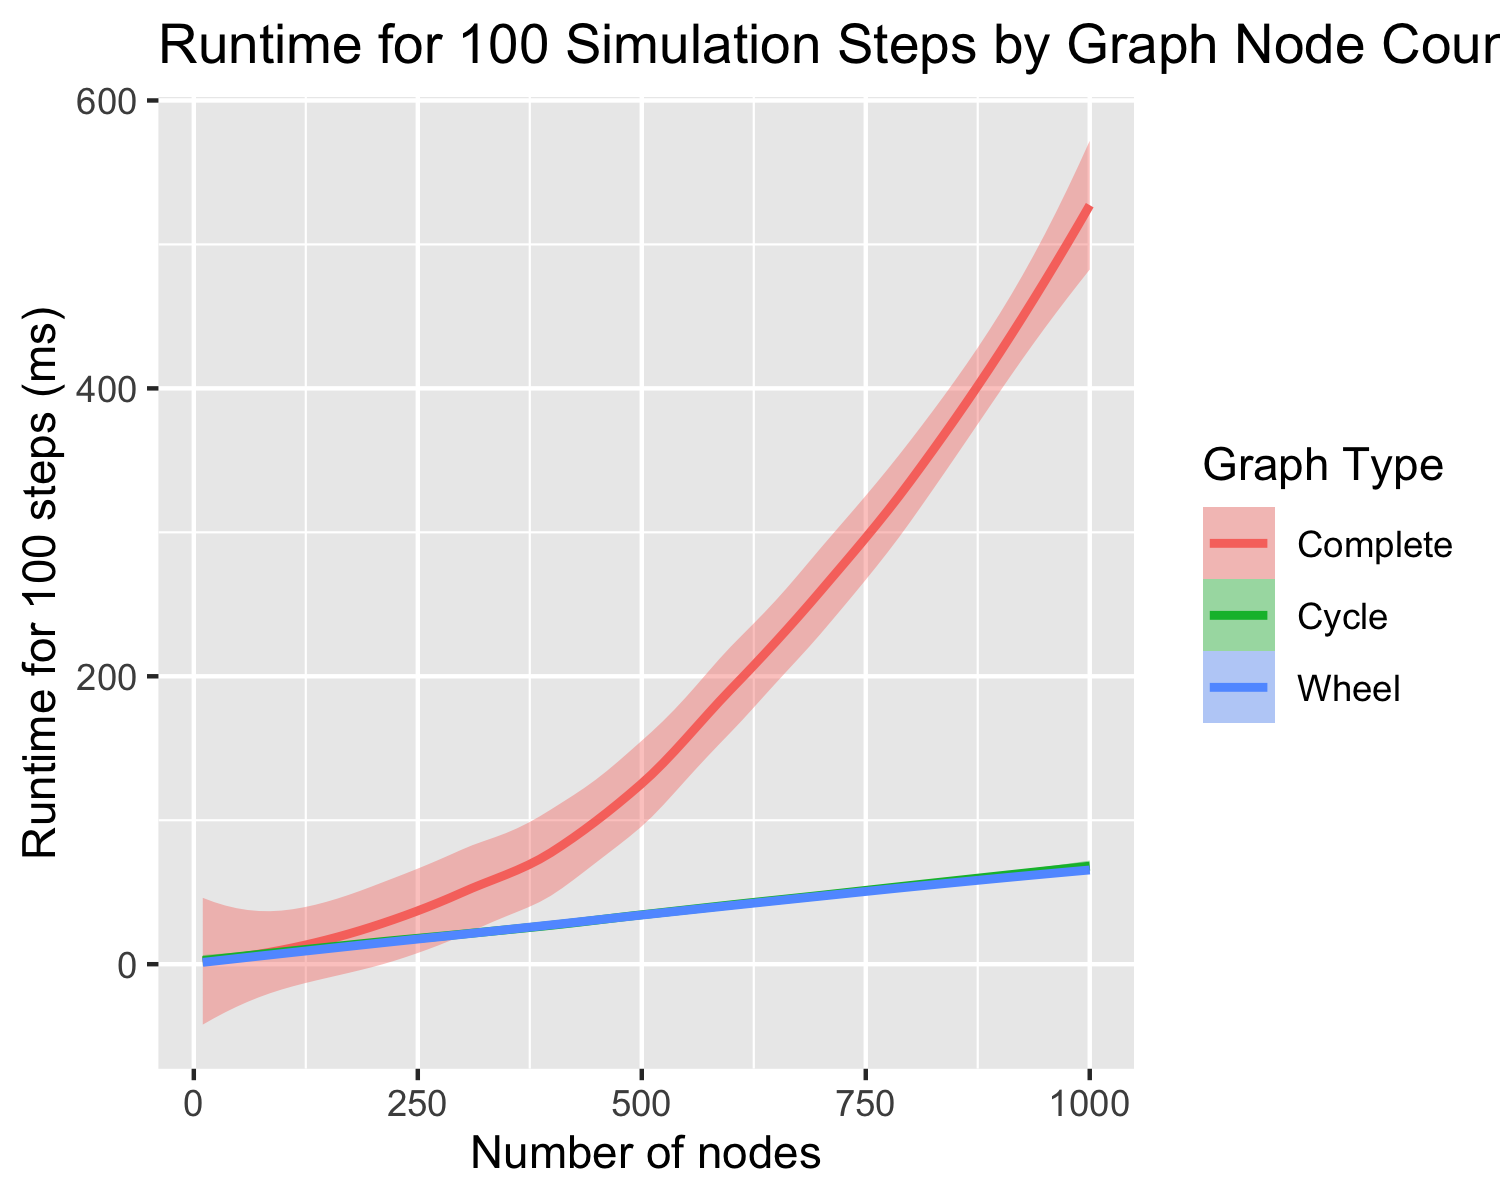
\includegraphics{figures/node_count_benchmarks.png}
\caption{Scaling is not linear in the number of agents (nodes). Note
that complete graphs, which have more edges, take much longer to step
than the wheel and cycle graphs which have fewer edges. The wheel and
cycle graphs take nearly the same time and
overlap.}\label{fig:nbenchmark}
}
\end{figure}

\begin{figure}
\hypertarget{fig:ebenchmark}{%
\centering
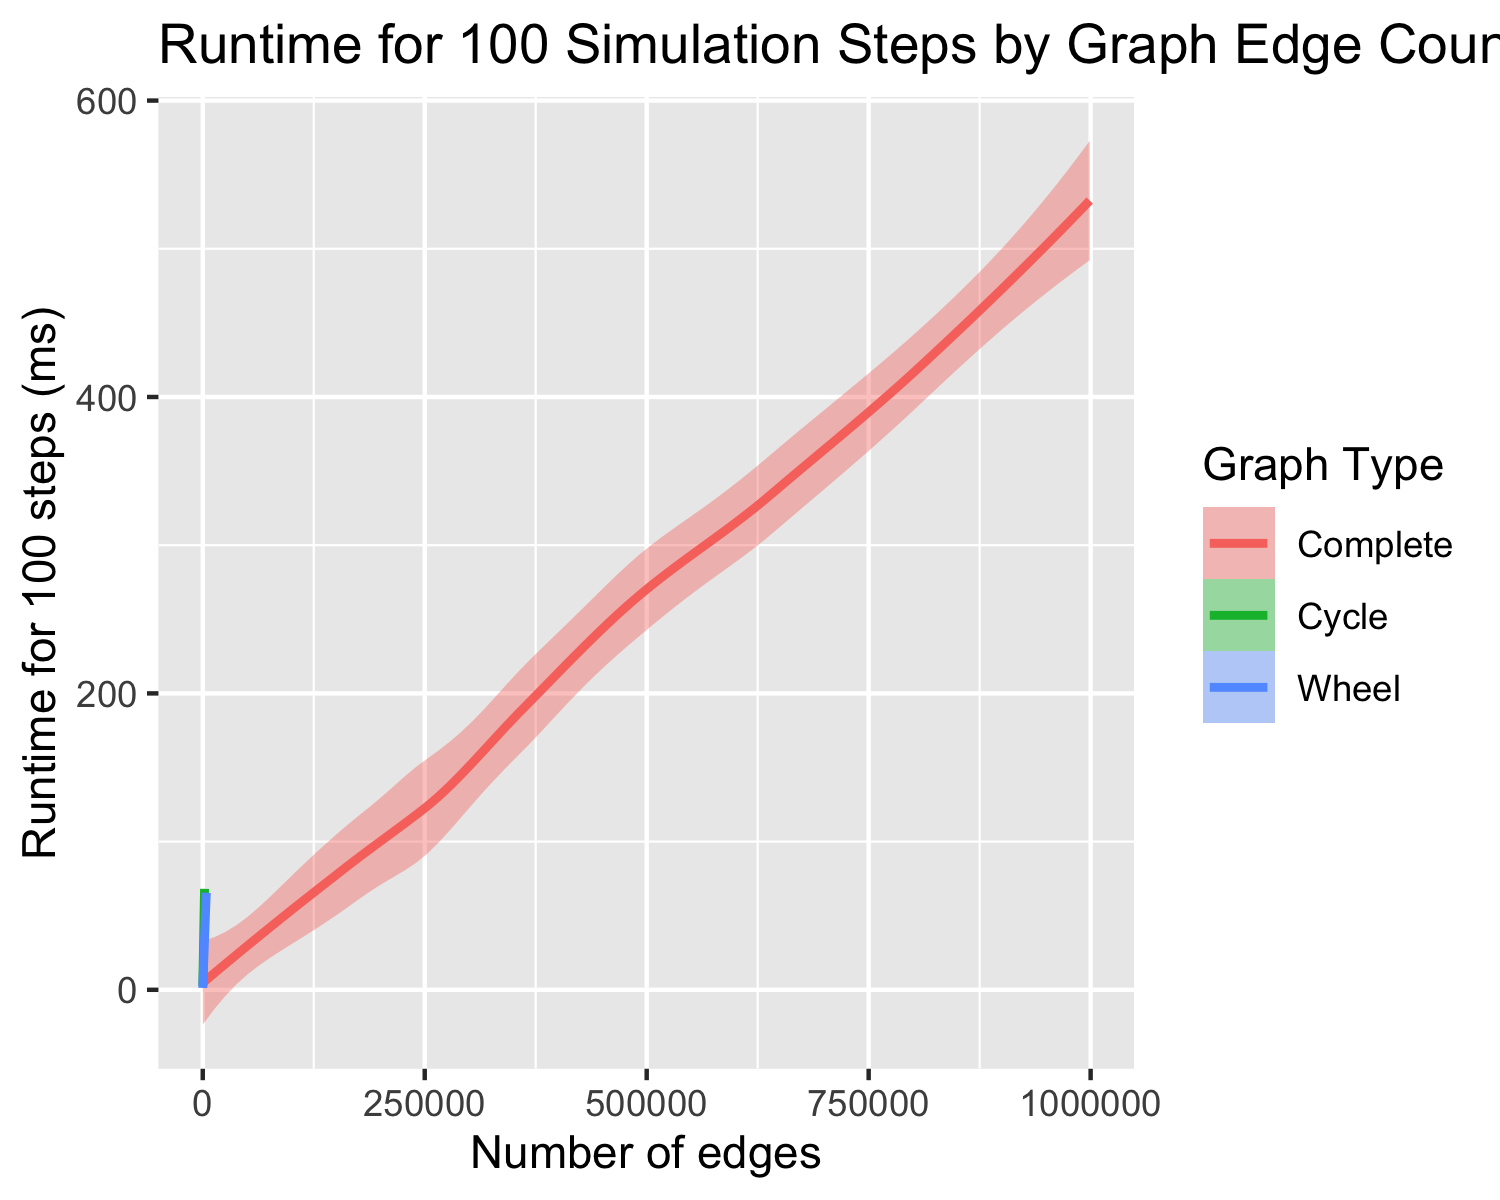
\includegraphics{figures/edge_count_benchmarks.png}
\caption{Scaling is linear in the number of edges as can be seen in the
complete graph scaling line. Note because the complete graph has many
more edges than the wheel and cycle graphs, it is difficult to see the
scaling curves for those graph times on this
graph.}\label{fig:ebenchmark}
}
\end{figure}


\hypertarget{crafting-empirically-motivated-social-network-models}{%
\chapter{Crafting Empirically-Motivated Social Network
Models}\label{crafting-empirically-motivated-social-network-models}}

Given the mechanistic interpretation I've given of Zollman's model in
\emph{The Epistemic Benefit of Transient Diversity}
\autocite{zollmanEpistemicBenefitTransient2009} and my account of how
mechanistic models can be evaluated based on how well the model's
mechanism represents that of the target's mechanism, I wish to
demonstrate how viewing models in this way leads to a more robust
evaluation of a model. Because making the entire model more
empirically-motivated would be a difficult undertaking, especially given
the model includes models of poorly-understood phenomena like belief
representations in people, I choose to focus on the model mechanism
Zollman focuses on: the network structure of scientists.

This experimental section then has two distinct parts: developing a
realistic and defensible model of network structure following from
empirical data and verifying that new model by attempting to replicate
Zollman's modeling results on these larger, more complex graphs. My
primary goal with this experimental work is less to evaluate Zollman's
model, but rather to present empirically-defined mechanism as another
way to evaluate mechanistic models in terms of empirical distance, as
discussed in previous sections. Viewed in opposition to Rosenstock et
al.'s critique of Zollman's model on the grounds that the results don't
hold outside a specific parameter range, my experimental work seeks to
determine how the model performs on parameter values determined by
empirical data, rather than mathematical idealizations. In short, if the
model mechanism looks a lot like the target mechanism, then how does
Zollman's model perform?

\hypertarget{graph-terminology}{%
\section{Graph Terminology}\label{graph-terminology}}

First, I will define some background terminology that is critical to
understanding both Zollman's models and my extensions of them.

A graph \(G\), mathematically, is a tuple \(G = (N, E)\) where \(N\) is
a set of \emph{nodes} and \(E\) is a set of tuples of vertices where
\((n_i, n_j) \in E\) represents an \emph{edge} or connection between
node \(n_i \in N\) and node \(n_j \in N\). Nodes are often also referred
to as vertices, however, I adopt Zollman's use of ``node'' for clarity
here. This structure of nodes and relations between nodes shows up in
many fields such as model theory in modal logics, biological modeling of
complex systems, and social network modeling. Graphs are very adept at
capturing relational structure in the real world, which brings up an
important distinction between \emph{graph} and \emph{network}. When I
say graph, I refer to the mathematical structure given above. A graph
has no interpretation, it is merely some structure made of nodes and
edges. A \emph{network}, on the other hand, refers to a relational
structure in the real world which can be modeled as a graph. For
example, if we want to model the internet as a graph (simplistically),
nodes might be computers, and edges might be network links between them.

Graphs may be \emph{directed} or \emph{undirected}. In a directed graph,
an edge represents a one-way connection where the edge \((n_i, n_j)\)
denotes a connection from \(n_i\) to \(n_j\) but not \(n_j\) to \(n_i\).
In an undirected graph, all edges are bidirectional such that
\((n_i, n_j)\) means both \(n_i\) connects to \(n_j\) and \(n_j\)
connects to \(n_i\). In practice, an undirected graph can be realized in
a directed graph so long as the edge \((n_i, n_j) \in E\) implies the
presence of the edge \((n_j, n_i) \in E\).

Because graph structure can be so rich, there are far more ways to
quantify structure than can be detailed and deployed in a single paper.
Instead, I will introduce a few fundamental properties that are
essential to understanding Zollman's model here. A connected graph is
one in which there exists a path connecting any two nodes in the graph,
where a path is defined as a sequence of nodes \(n_1, \ldots, n_l\) such
that for each \(n_i\) in the path, there exists an edge
\((n_i, n_{i+1}) \in E\). In an undirected graph, the order of an edge
is ignored. For directed graphs, there are two senses of connectivity
\emph{weak} and \emph{strong}. Weak connections treat the directed graph
as undirected (ignoring the direction of edges) whereas strong
connections do not.

To illustrate these definitions, consider the following directed graph
\((N, E) = \left(\{ 1, 2, 3 \}, \{ (1, 2), (1, 3) \}\right)\). The graph
is weakly connected (and thus connected if undirected) because the node
\(1\) is connected to node 2 via \((1, 2)\) and to node 3 via
\((1, 3)\). Node 2 is connected to node \(1\) via \((1, 2)\) and to node
3 via \((1, 2)\) and \((1, 3)\). Node 3, similarly to node 2, is
connected to node \(1\) via \((1, 3)\) and to node 3 via \((1, 3)\) and
\((1, 2)\). Note that nodes 2 and 3 do no connect to any other node if
edges are instead directed. Thus, this graph is weakly connected, but
not strongly connected.

Finally, this definition of connectivity leads to the idea of
\emph{connected components} when combined with the idea of a
\emph{subgraph}. A \emph{subgraph} \(G' = (N', E')\) of a graph
\(G = (N, E)\) is formed by a subset of nodes \(N' \subseteq N\) and and
a subset of edges \(E' \subseteq E\) such that \(E'\) contains only
edges where both endpoints are in \(N'\). Now, a connected component is
a subgraph of \(G\) such that \(G'\) is connected. In addition, if the
\(G\) is directed and all nodes in \(G'\) is a strongly connected graph,
then \(G'\) is a strongly connected component of \(G\). Conversely, if
\(G'\) fits the definition of a weakly connected graph, then \(G'\) is a
weakly connected component.

Finally, there are several types of ideal graphs that are often
discussed and that Zollman uses as test cases in his paper. First, a
\emph{complete} graph is one in which every node is connected to every
other node in a graph. Second, a \emph{cycle} is a strongly connected
graph in which every node is connected to exactly two neighbors such
that all nodes are connected in one large ring. Finally a \emph{wheel}
is a strongly connected graph identical to a cycle, with the addition of
a single central node that is connected to every other node.

\hypertarget{zollmans-communication-networks}{%
\section{Zollman's Communication
Networks}\label{zollmans-communication-networks}}

While I will not rehash my framing of Zollman's model mechanistically in
this section, I will spend a bit of time focusing on the technicalities
of how the network structure part of the model operates. I'll begin with
a discussion of the intended target of Zollman's model to clarify what a
charitable interpretation of his work might be, before discussing how
this intention is represented in the actual model machinery.

Zollman discusses social networks, where he defined individuals as nodes
and edges to be the ``the communication of results from one to the
other'' \autocite[p.~25][]{zollmanEpistemicBenefitTransient2009}.
Furthermore, he posits that this relationship is symmetric, so if an
individual \(A\) can view individual \(B\)'s results, \(B\) can also
view \(A\)'s results. This definition can mean quite a few things in
practice and will prove too broad to apply directly to measurable
real-world behaviors. To demonstrate this, consider the following cases
where results are communicated:

\begin{enumerate}
\def\labelenumi{\arabic{enumi}.}
\tightlist
\item
  A scientist reads a published work, finds the results interesting, and
  eventually cites that work in her own work building off of or
  criticizing the published work.
\item
  A scientist reads a published journal article, finds the results
  uninteresting, and does not ever cite the work.
\item
  A scientist reads a news article about some research work, is
  influenced by the high-level ideas, but never reads underlying
  academic work, and thus does not cite it.
\item
  A scientist emails a friend in another lab for advice about starting a
  project and the friend reports that their results in the project area
  didn't look promising. Nothing is published, but info about results is
  transmitted.
\item
  A prominent scientist writes a blog or tweet reacting to a paper,
  influencing people's opinions of that paper without any published work
  to document it.
\item
  A scientist runs into another researcher at a conference and the two
  informally share ideas.
\end{enumerate}

Beyond these, there many other ways by which results may be communicated
within a scientific community with varying degrees of impact and
evidence associated with the transfer. Many of the more informal methods
of communication would be very hard to measure or quantify on a large
scale. Informal conversations and emails are rightly private and not
available for public analysis and social media is an emerging form of
communication for scientists which is not yet well-understood
\autocite{collinsHowAreScientists2016a}. Thus, these forms of
communication of results are difficult to measure and quantify.

Citations, on the other hand, formally recognize the specific results of
prior work which influenced the researcher. The APA's influential
publication manual formalizes this influence-based understanding of
citation, recommending that researchers ``cite the work of those
individuals whose ideas, theories, or research have directly influenced
your work'' \autocite{PublicationManualAmerican2010}. These citations
often take on a more strategic rhetorical purpose, explicitly building
on a paradigm of work started by another or criticizing that paradigm.
This argumentative conception of a citation's role in a scientific
community is characterized in greater depth by Bruno Latour in
\emph{Science in Action} as a part of his Actor-Network theory
\autocite{latourLiterature1987a}. However, for our purposes, we need not
wade into the subtleties here because no matter how a citation is
deployed in this sense, it trivially can be said to have influenced the
author. Even if the author is just cursorily familiar with the work and
is citing to criticize the approach, they display some awareness of the
results found. Citations don't always live up to this intent, as authors
may cite simply to help get by publication referees, and in some cases,
journals even force authors to cite certain articles, forming ``coercive
citations'' \autocite{wilhiteCoerciveCitationAcademic2012}. Despite
these degenerate cases, I argue it is fairly safe to assume that a
majority of authors who cite can be accurately described as receiving
and considering results from another party.

However, the reason to focus on citations over other forms of
communication is that citations do have norms which seem to be followed
to some extent and, critically, they are measurable empirically as a
result of the collection and systematization of academic metadata. While
I'll go into the practicalities of how in the next section, citation and
author data is easily available for large-scale analysis across nearly
every field of study. Because this data directly represents real
scientists citing the work of others, it has the potential to serve as a
convincing stand-in for what the real-world scientific communities might
look like.

So to create a more realistic account of network structure in science, I
plan to start from this data, rather than from the idealized graphs
Zollman proposed. The hope here is not that this data will prove a
perfect proxy for real communication, as no single data source captures
the full breadth of human communication, but as a much more
empirically-motivated structure than Zollman's rings, cycles and
complete graphs. However, to effectively deploy citation metadata to
create realistic communication structures, I must create a reasonable
rule for what constitutes evidence of communication and thus when to
draw an edge.

\hypertarget{constructing-realistic-graphs}{%
\section{Constructing Realistic
Graphs}\label{constructing-realistic-graphs}}

I divide this section into three distinct parts. First, I detail why I
selected the Microsoft Academic Graph (MAG) and what specific data it
contains. Then, I briefly detail my strategy for processing the large
dataset and finally conclude with a more formal definition of how I
define communication in terms of the specific metadata present in the
MAG.

\hypertarget{comprehensive-metadata}{%
\subsection{Comprehensive Metadata}\label{comprehensive-metadata}}

To infer communication from an academic social network, we first begin
with a comprehensive dataset of academic publishing metadata. By
publishing metadata, I refer to all the data associated with a scholarly
journal article, conference paper, or book except for the actual text of
the work itself. A good way to think about such metadata is everything
found on a ``works cited'' page: the title, a list of authors, the date
of publication, the journal, etc. However, most datasets also go beyond
this metadata and also include a set of citation links to other papers,
a set of fields of study as assigned by publishers as well as links to
other works that reference that paper.

Luckily several comprehensive sources of this metadata exist. Clarivate
Analytics compiles ``Web of Science'' (WoS), a proprietary dataset that
has vetted and comprehensive scientific metadata spanning from 1900 to
the present and including over 200 million entries. However, I decided
against using this dataset, which is commonly used in bibliometric
papers which analyze citation metadata, due to the closed nature of the
dataset which create barriers for researchers. There is also a young
project, OpenCitations, which seeks to build a citation data repository
that is entirely open with vetted data from publishers, however, the
project is still young and coverage sparse covering fewer than half a
million works
\autocite{peroniOpenCitationsInfrastructureOrganization2020}. For this
project, I chose to use the MAG
\autocite{sinhaOverviewMicrosoftAcademic2015b,wangReviewMicrosoftAcademic2019}
which leverages Bing's web indexing service much like Google Scholar
leverages Google's search infrastructure to generate a comprehensive
account of academic metadata, covering over 170 million entities.
However, unlike WoS, the data is available under a permissible license
(the Open Data Commons Attribution License) at no cost to the
researcher. This drove me to select the MAG over the others because it
presents the fewest barriers to follow on work and allows me to make my
results freely available.

\hypertarget{processing-a-large-graph}{%
\subsection{Processing a Large Graph}\label{processing-a-large-graph}}

The specific data in the MAG is evolving constantly, however, I use a
snapshot taken in October of 2018 for all my analysis. My MAG snapshot
is a ``multi-graph'' or a graph with different node types for authors
(\texttt{Author}), papers (\texttt{Paper}), fields of study
(\texttt{FieldOfStudy}) and journals (\texttt{Journals}). Furthermore,
there are directed edges for citations which connect papers to papers by
their listed citations (\texttt{REFERENCES}), from papers to their
authors (\texttt{AUTHORED\_BY}), from papers to their fields of study
(\texttt{IN\_FIELD}), and from subfields to their parent fields
(\texttt{PARENT}). These relations are formatted as a series of very
large CSV files (10-100GB each) and are not easily searchable in their
raw form as a result. Such large files do not fit in RAM on any
affordable machine, meaning it is not feasible to use the graph in its
entirety for simulations. Furthermore, understanding and visualizing the
results of a simulation of such a large size would be a difficult
undertaking.

To make this data useable, I decided to use the popular graph database
neo4j \autocite{Neo4j} to quickly query for smaller chunks of the
overall graph. While queries over most of the properties and relations
in the MAG are possible, I decided to focus on returning edges which
represent probable paths of communication between authors. To get this
large dataset into neo4j, I needed to convert the relations from the raw
tab-separated CSV files (TSV) to CSVs, then use the offline importer to
neo4j. To do this, I built a small conversion program in the programming
language Rust (\texttt{mag-csv} in source code) which could perform the
conversions quickly. I then fed the output of this conversion program
into neo4j's offline bulk import tool (\texttt{neo4j-import}) which
efficiently imported the data. I took this route because importing via
traditional queries is far too slow to be feasible for a dataset of this
size (the ``fast'' import still took several days on a laptop with a
relatively fast solid-state storage drive).

\hypertarget{the-authorcites-relation}{%
\subsection{\texorpdfstring{The \texttt{AuthorCites}
Relation}{The AuthorCites Relation}}\label{the-authorcites-relation}}

Once the data was in query-able form, I turned my focus to determining
the precise relations I would use to capture likely communication
relations between authors. To do this, I wanted to leverage citations
because they are instances where we have clear evidence in the MAG that
one work has influenced another. However, citations relate papers, not
authors, so the cited relation must be lifted to apply to authors.
Consider two authors \(A_1\) and \(A_2\). We say that \(A_1\) cites
\(A_2\) if and only if there exist papers \(P_1\) and \(P_2\) such that
\(A_1\) authored \(P_1\), \(P_1\) cites \(P_2\) and \(A_2\) authored
\(P_2\). Formally:

\begin{align*}
\texttt{AuthorCites}(A_1, A_2) = \exists_{ P_1, P_2 \in \texttt{Papers} } (                &\texttt{AUTHORED\_BY} (P_1, A_1) \land \\
   &\texttt{REFERENCES}(P_1, P_2) \land \\
   &\texttt{AUTHORED\_BY}(P_2, A_2) )
\end{align*}

All that is required is that a single pair of papers \(P_1\) and \(P_2\)
exist to maintain the \texttt{AuthorCites} relation. From this relation,
we infer that results were communicated from \(A_2\) to \(A_1\) by way
of \(A_1\) reading or reacting to \(A_2\)'s work, which indicates both a
general awareness of the cited author and the results presented in the
paper. This may be a cursory awareness if the citing author glanced at
the cited paper before using the citation strategically, however, that
is still transmitted information which could alter the direction of the
author's research. This is no perfect relation because many types of
communication happen without a subsequent citation. Furthermore,
citations themselves might represent little to no information
transferred. However, I argue that this method does a much better job of
approximating scientific community structure than a cycle, wheel,
complete or any other idealized graph would by virtue of being derived
from real data about real interactions.

An important point of comparison here is the co-authorship relation
which is often used in bibliometric community analysis. This simply
connects two authors when they have co-authored a paper together. While
co-authorship is a strong signal that information has been transmitted,
I argue it is overly restrictive to fit well with Zollman's definition
of edges representing communication of results between two parties.
Furthermore, when there is a sole author, co-authorship would not
reflect any other community members that the sole author was influenced
by. This feels wrong, especially when the author cited other papers, so
I chose to go with the \texttt{AuthorCites} relation.

While the \texttt{AuthorCites} relation does capture what we want at a
high level, it does not help limit the overall data processed in a given
query. To do this, I create the \texttt{AuthorCitesInField} which limits
connections to only those in which \(P_1\) and \(P_2\) are both in the
field of study of interest, \(F \subseteq \text{Papers}\). Thus, the
definition becomes:

\begin{align*}
\texttt{AuthorCites}(A_1, A_2) = \exists_{ P_1, P_2 \in F } (                &\texttt{AUTHORED\_BY} (P_1, A_1) \land \\
   &\texttt{REFERENCES}(P_1, P_2) \land \\
   &\texttt{AUTHORED\_BY}(P_2, A_2) )
\end{align*}

Because we are focused on specific communities, this definition works
well while significantly reducing query complexity by only quantifying
over every paper within a single field, rather than over every last
paper in the MAG. This does ignore interdisciplinary work, which is an
unfortunate downside to this approach, however, the decrease in query
complexity achieved here is what makes these queries feasible at all
using a relatively small machine.

Given the definition of \texttt{AuthorCitesInField}, I crafted the
following neo4j query. The query takes on a different form than the
definition to better leverage the graph structure and relations that
exist in the graph. There is no relation which links authors to fields
of study, so it is much faster in practice to enumerate a list of papers
in a field than a list of authors. This query, as written, will result
in duplicate relationships between authors, however, those are more
effectively de-duplicated in a graph processing library rather than in
the database.

\begin{verbatim}
MATCH (p1:Paper)-[:IN_FIELD]->(parent:FieldsOfStudy{id: $id})
WHERE p1.citationCount > 0
MATCH (p1:Paper)-[r:REFERENCES]->(p2:Paper)
MATCH (p2:Paper)-[:IN_FIELD]->(parent:FieldsOfStudy{id: $id})
WHERE p2 <> p1 AND p2.citationCount > 0
MATCH (p2:Paper)-[:AUTHORED_BY]->(a2:Author)
MATCH (p1:Paper)-[:AUTHORED_BY]->(a1:Author)
WHERE a1 <> a2
RETURN a1, a2
\end{verbatim}

\hypertarget{selecting-subgraphs}{%
\section{Selecting Subgraphs}\label{selecting-subgraphs}}

Now that I've described my method for relating authors via citations, I
tried the method out on several areas of research. To pick a diverse set
of fields of research, I used the MAG's fields of study as groupings and
its hierarchical organization of fields of study to select fields to
analyze. This organization places each field in a tree that descends
from a ``root'' field which has no parent.

I started by selecting ``social epistemology'' and ``peptic ulcer''. I
choose these two because Zollman publishes in the field of social
epistemology and writes about the field of peptic ulcer research in his
case study. After selecting these, I chose ``brain morphometry'' as a
subfield of neuroscience, ``monetary policy'' as a subfield of
economics, ``abstract algebra'' as a subfield of math and ``phonetics''
as a subfield of linguistics. My goal with this selection of fields is
to find fields of different sizes and with likely somewhat different
citation practices and cultures to ensure that my tests of Zollman's
model do not result in field-specific results.

In Tables \ref{tbl:networknec} and \ref{tbl:networkscc}, I detail the
resulting \texttt{AuthorCitesInField} graphs in relation to
co-authorship graphs, which serve as a point of comparison. I report
node and edge counts to give a general idea of the size of a field in
Table \ref{tbl:networknec}, where nodes are authors and edges are
\texttt{AuthorCitesInField} relations which connect authors to author's
they've cited via directed edges. Thus, the more nodes, the bigger the
field and the more edges, the more well connected the field. I report
basic stats pertaining to the connected components (both strong and
weak) in Table \ref{tbl:networkscc}. This includes both a count of the
total number of separate components as well as the size of the largest
one. It is important to note that because co-authorship is undirected,
strong and weak connectivity are the same for those networks.
Connectivity is a crude measure of the cohesion of a community which
partition the graph into sections such that no edge goes between
sections. These partitions of the graph represent fractures in the
community such that authors in separated components have never cited
anyone in any of the other sections. Having many large components
suggests either that fields are themselves fractured or that the MAG
mislabeled some author's work, leading them to be an island in a
spuriously assigned field. For larger, broader fields, it makes sense
that the field would be partitioned as it seems more likely that
research might be labeled under that field without much connection to
the primary body of work for the field.

A striking characteristic of most of the \texttt{AuthorCitesInField} and
co-authorship fields is the emergence of singular large weakly connected
components that contain most of the nodes in many, but not all, of the
selected fields. However, in nearly all cases, the weakly connected
component is much larger than the strongly connected component. This
effect is commonly observed in large graphs and most famously first
observed in the analysis of the early web
\autocite{broderGraphStructureWeb2000b}, where the large weakly
connected component did not imply a large strongly connected component.
These results emphasize the structural differences between directed and
undirected graphs, in that simply allowing the
\texttt{AuthorCitesInField} to be bidirectional can unify a fractured
field. Because Zollman's models are only meant to be run on connected
graphs, the model will, in practice, be run on connected subgraphs
rather than the overall fields.

\begin{longtable}[]{@{}lrr@{}}
\caption{Selected fields and resulting \texttt{AuthorCitesInField}
networks and Co-Authorship and associated node and edge counts.
\label{tbl:networknec}}\tabularnewline
\toprule
network & nodes & edges\tabularnewline
\midrule
\endfirsthead
\toprule
network & nodes & edges\tabularnewline
\midrule
\endhead
social epistemology AuthorCited & 651 & 1490\tabularnewline
social epistemology CoAuthor & 1663 & 3777\tabularnewline
brain morphometry AuthorCited & 5154 & 77371\tabularnewline
brain morphometry CoAuthor & 8584 & 139059\tabularnewline
monetary policy AuthorCited & 17620 & 454030\tabularnewline
monetary policy CoAuthor & 30418 & 108882\tabularnewline
abstract algebra AuthorCited & 311 & 968\tabularnewline
abstract algebra CoAuthor & 977 & 2400\tabularnewline
peptic ulcer AuthorCited & 20970 & 562167\tabularnewline
peptic ulcer CoAuthor & 49017 & 317141\tabularnewline
phonetics AuthorCited & 5766 & 58192\tabularnewline
phonetics CoAuthor & 10399 & 36707\tabularnewline
\bottomrule
\end{longtable}

\begin{longtable}[]{@{}lrrrr@{}}
\caption{Selected fields and resulting \texttt{AuthorCitesInField} (AC)
networks and Co-Authorship (CA) and associated strongly connected
component (SCC) counts, weakly connected component (WCC) counts, the
size of the largest strongly connected component, and the size of the
largest weakly connected component.
\label{tbl:networkscc}}\tabularnewline
\toprule
network & largest SCC & num SCCs & largest WCC & num WCCs\tabularnewline
\midrule
\endfirsthead
\toprule
network & largest SCC & num SCCs & largest WCC & num WCCs\tabularnewline
\midrule
\endhead
social epistemology AC & 10 & 615 & 560 & 30\tabularnewline
social epistemology CA & 82 & 596 & 82 & 596\tabularnewline
brain morphometry AC & 1661 & 3392 & 5049 & 11\tabularnewline
brain morphometry CA & 5186 & 576 & 5186 & 576\tabularnewline
monetary policy AC & 9616 & 7913 & 17541 & 32\tabularnewline
monetary policy CA & 13306 & 5974 & 13306 & 5974\tabularnewline
abstract algebra AC & 12 & 285 & 192 & 29\tabularnewline
abstract algebra CA & 25 & 337 & 25 & 337\tabularnewline
peptic ulcer AC & 8383 & 12444 & 20449 & 67\tabularnewline
peptic ulcer CA & 14698 & 7371 & 14698 & 7371\tabularnewline
phonetics AC & 2049 & 3640 & 5608 & 29\tabularnewline
phonetics CA & 3734 & 2064 & 3734 & 2064\tabularnewline
\bottomrule
\end{longtable}


\hypertarget{evaluating-empirically-motivated-network-models}{%
\chapter{Evaluating Empirically-Motivated Network
Models}\label{evaluating-empirically-motivated-network-models}}

\usetikzlibrary{positioning,arrows,calc}
\tikzset{
    graph/.style={>=stealth,shorten >=1pt,shorten <=1pt,auto,node distance=1.5cm, semithick},
    world/.style={circle,draw,minimum size=0.5cm,fill=gray!15}, point/.style={circle,draw,inner sep=0.5mm,fill=black},
    model/.style={circle,draw,minimum size=0.5cm,fill=gray!20}, point/.style={circle,draw,inner sep=0.5mm,fill=black},
    reflexive above/.style={->,loop,looseness=7,in=120,out=60},
    reflexive below/.style={->,loop,looseness=7,in=240,out=300},
    reflexive left/.style={->,loop,looseness=7,in=150,out=210},
    reflexive right/.style={->,loop,looseness=7,in=30,out=330}
}

In this section, I turn my attention to actually using these
citation-based networks to evaluate Zollman's modeling efforts. It is
divided into three distinct investigations which each answer one of the
following questions:

\begin{enumerate}
\def\labelenumi{\arabic{enumi}.}
\tightlist
\item
  How does social network graph structure differ from the idealized
  models used by Zollman?
\item
  How do Zollman's results hold up on social network structure?
\item
  How can the new model behavior be characterized?
\end{enumerate}

\hypertarget{examining-graph-structure}{%
\section{Examining Graph Structure}\label{examining-graph-structure}}

The goal of this part is to show that there are important differences
between the MAG-derived empirical graphs and the canned cycle, wheel,
and complete graphs found in Zollman. However, before comparing these
graphs we must ensure that the output from the MAG from the prior
section fulfills all the requirements to work for the Bala-Goyal models
Zollman uses.

A key requirement of Bala-Goyal models is that the network is connected.
That is, every node can reach every other node. Intuitively, this is a
fine stipulation as an unreachable node is clearly outside of any
community represented by a graph. This can be seen in Figure
\ref{fig:disjoint} where two disjoint subgraphs \(A\) and \(B\) can be
separable from the combined graph \(A \cup B\).

\begin{figure}
    \centering
    \begin{tikzpicture}[graph]
        \node[world] (a1) {$a_1$};
        \node[world] (a2) [below right=of a1] {$a_2$};
        \node[world] (a3) [below left=of a1] {$a_3$};

        \node[world] (b2) [right=of a2] {$b_2$};
        \node[world] (b3) [above right=of b2]{$b_3$};
        \node[world] (b1) [above left=of b2]{$b_1$};

        \path[->] (b1) edge (b2);
        \path[->] (b2) edge (b3);
        \path[->] (b3) edge (b1);
        \path[->] (a1) edge (a2);
        \path[->] (a2) edge (a3);
        \path[->] (a3) edge (a1);

    \end{tikzpicture}
    \caption{Two disconnected graphs, $A = \{ a_1, a_2, a_3 \}$, $B = \{ b_1, b_2, b_3 \}$. If we are studying the combined graph $A \cup B$, we'd be better off splitting the graph into $A$ and $B$ to be studied separately.}
    \label{fig:disjoint}
\end{figure}

The example in figure \ref{fig:disjoint} doesn't pose any issues for any
simulation run because both graphs will simply run independently, but
still correctly. However, problematic structures do commonly occur in
the MAG where information doesn't propagate or propagates only in one
direction, likely as a result of missing citations in the metadata.
Figure \ref{fig:isolate} demonstrates what this might look like where
isolated nodes would have no network effects and instead only rely on
their own random sampling. In practice, because agents are myopic and
pick whatever they think is successful, the initial random seed will
dictate the final action chosen because no data from neighbors ever
comes in.

\begin{figure}
    \centering
    \begin{tikzpicture}[graph]
        \node[world] (a1) {$a_1$};
        \node[world] (a2) [below right=of a1] {$a_2$};
        \node[world] (a3) [below left=of a1] {$a_3$};

        \node[world] (b1) [right=of a2] {$b_1$};
        \node[world] (b2) [above right=of b2]{$b_2$};
        \node[world] (c1) [above left=of b2]{$c_1$};

        \path[->] (b1) edge (b2);
        \path[->] (a1) edge (a2);
        \path[->] (a2) edge (a3);
        \path[->] (a3) edge (a1);

    \end{tikzpicture}
    \caption{Three disconnected graphs, $A = \{ a_1, a_2, a_3 \}$, $B = \{ b_1, b_2\}$, $C = \{c_1\}$. In this case, $c_1$ and $b_1$ experience no network effects at all because they have no neighbors.}
    \label{fig:isolate}
\end{figure}

To avoid these effects, I needed a construction that can take the
fragmented, large graphs and return the connected communities which lie
within them. The strongly connected component definition turned out to
be just that. If we recall from the previous section, a strongly
connected component is a subgraph of a larger graph where all nodes in
the subgraph are mutually reachable. In a strongly connected component,
every node has a neighbor. This stands in contrast to a weakly connected
component where all nodes simply must be reachable by some other node.
In the undirected graphs that Zollman used, these two definitions are
equivalent, however, because the citation relation is directed, I opt
for the strongly connected component to preserve the property that every
node has a neighbor. See Figure \ref{fig:3} for an example.

\begin{figure}
    \centering
    \begin{tikzpicture}[graph]
        \node[world] (a1) {$a_1$};
        \node[world] (a2) [below right=of a1] {$a_2$};
        \node[world] (a3) [below left=of a1] {$a_3$};

        \node[world] (b1) [right=of a2] {$b_1$};
        \node[world] (b2) [above right=of b2]{$b_2$};

        \path[->] (b1) edge[bend right] (b2);
        \path[->] (b2) edge[bend right] (b1);
        \path[->] (a2) edge (b1);
        \path[->] (a1) edge (a2);
        \path[->] (a2) edge (a3);
        \path[->] (a3) edge (a1);
    \end{tikzpicture}
    \caption{Strongly connected components are $A = \{ a_1, a_2, a_3 \}$ and $B = \{ b_1, b_2 \}$ whereas $A \cup B$ is a weakly connected component}
    \label{fig:3}
\end{figure}

So, given this definition, I further refine my graphs to be the strongly
connected components present in the field-specific graphs returned from
the MAG. As noted in the earlier section, there can be many strongly
connected components in a single field and these components can be quite
large. So, how do these components compare to the graphs Zollman used?
Figure \ref{fig:4} has examples of the cycle, wheel, and complete graphs
for reference. Note that these graphs can be scaled to any size
following the same patterns.

\begin{figure}
    \centering
    \begin{tikzpicture}[graph]
        \node[world] (a1) {$a_1$};
        \node[world] (a2) [right=of a1] {$a_2$};
        \node[world] (a3) [below=of a2] {$a_3$};
        \node[world] (a4) [below=of a1] {$a_4$};

        \node[world] (b1) [right=of a2] {$b_1$};
        \node[world] (b2) [right=of b1] {$b_2$};
        \node[world] (b3) [below=of b1] {$b_3$};
        \node[world] (b4) [below=of b2] {$b_4$};

        \node[world] (c1) [right=of b2] {$c_1$};
        \node[world] (c3) [below right=of c1] {$c_3$};
        \node[world] (c2) [above right=of c3] {$c_2$};
        \node[world] (c4) [below left=of c3] {$c_4$};
        \node[world] (c5) [below right=of c3] {$c_5$};

        \path[<->] (a1) edge (a2);
        \path[<->] (a2) edge (a3);
        \path[<->] (a3) edge (a4);
        \path[<->] (a4) edge (a1);

        \path[<->] (b1) edge (b2);
        \path[<->] (b1) edge (b3);
        \path[<->] (b1) edge (b4);
        \path[<->] (b2) edge (b3);
        \path[<->] (b2) edge (b4);
        \path[<->] (b3) edge (b4);
        \path[<->] (b4) edge (b1);

        \path[<->] (c1) edge (c2);
        \path[<->] (c2) edge (c5);
        \path[<->] (c5) edge (c4);
        \path[<->] (c4) edge (c1);
        \path[<->] (c1) edge (c3);
        \path[<->] (c2) edge (c3);
        \path[<->] (c4) edge (c3);
        \path[<->] (c5) edge (c3);
    \end{tikzpicture}
    \caption{Cycle $A = \{ a_1, a_2, a_3, a_4\}$, complete $B = \{ b_1, b_2, b_3, b_4 \}$ and wheel $C = \{ c_1, c_2, c_3, c_4, c_5 \}$}
    \label{fig:4}
\end{figure}

Now, given this understanding, I turn my attention back to understanding
how these collections of strongly-connected components from the
AuthorCites differ structurally from the synthetic graphs. The point of
this examination is to provide context that helps us understand the
simulation results as this structure should lead to those results.

To show how the wheel, cycle, and complete graphs differ, I first
created a scatter plot in Figure \ref{fig:nodesvdensity} which relates
the number of nodes and the density in each graph. Density is defined as
the number of actual edges over the number of potential edges in the
graph if it were a complete graph. The goal of plotting this
relationship is to ask if these empirical graphs have a similar
structure to any one of the synthetic graphs. Because complete graphs
are far denser than cycle and wheel graphs, I plotted this relationship
on a \(\log\)-\(\log\) plot to better visualize the differences between
them.

As it turned out, larger empirical graphs become much less dense as they
increase in size and are much closer to wheel graphs than to complete
graphs. Many fall in the wide region between wheel graphs and complete
graphs, indicating that there are many real communities in science which
have quite different density and structure than the synthetic graphs
discussed by Zollman. Furthermore, these differences grow as these
communities become larger because the quadratic growth of complete
graphs diverges from the more limited number of connections that any
given researcher could have.

What is important about this result is that the complete graph should be
regarded as a fairly unrealistic structure within larger research
communities. This result makes a lot of intuitive sense: as a community
grows in size, the ability of a single person to meaningfully read and
engage with others remains fixed. In a ten-person community, an author
might be able to read papers by everyone within that community, whereas
in a ten thousand person community authors will only be able to read,
let alone cite, a small fraction of that community. Thus, this
demonstrates that in the large communities that dominate today's global
research community, Zollman's dense complete networks are quite
unrealistic.

\begin{figure}
\hypertarget{fig:nodesvdensity}{%
\centering
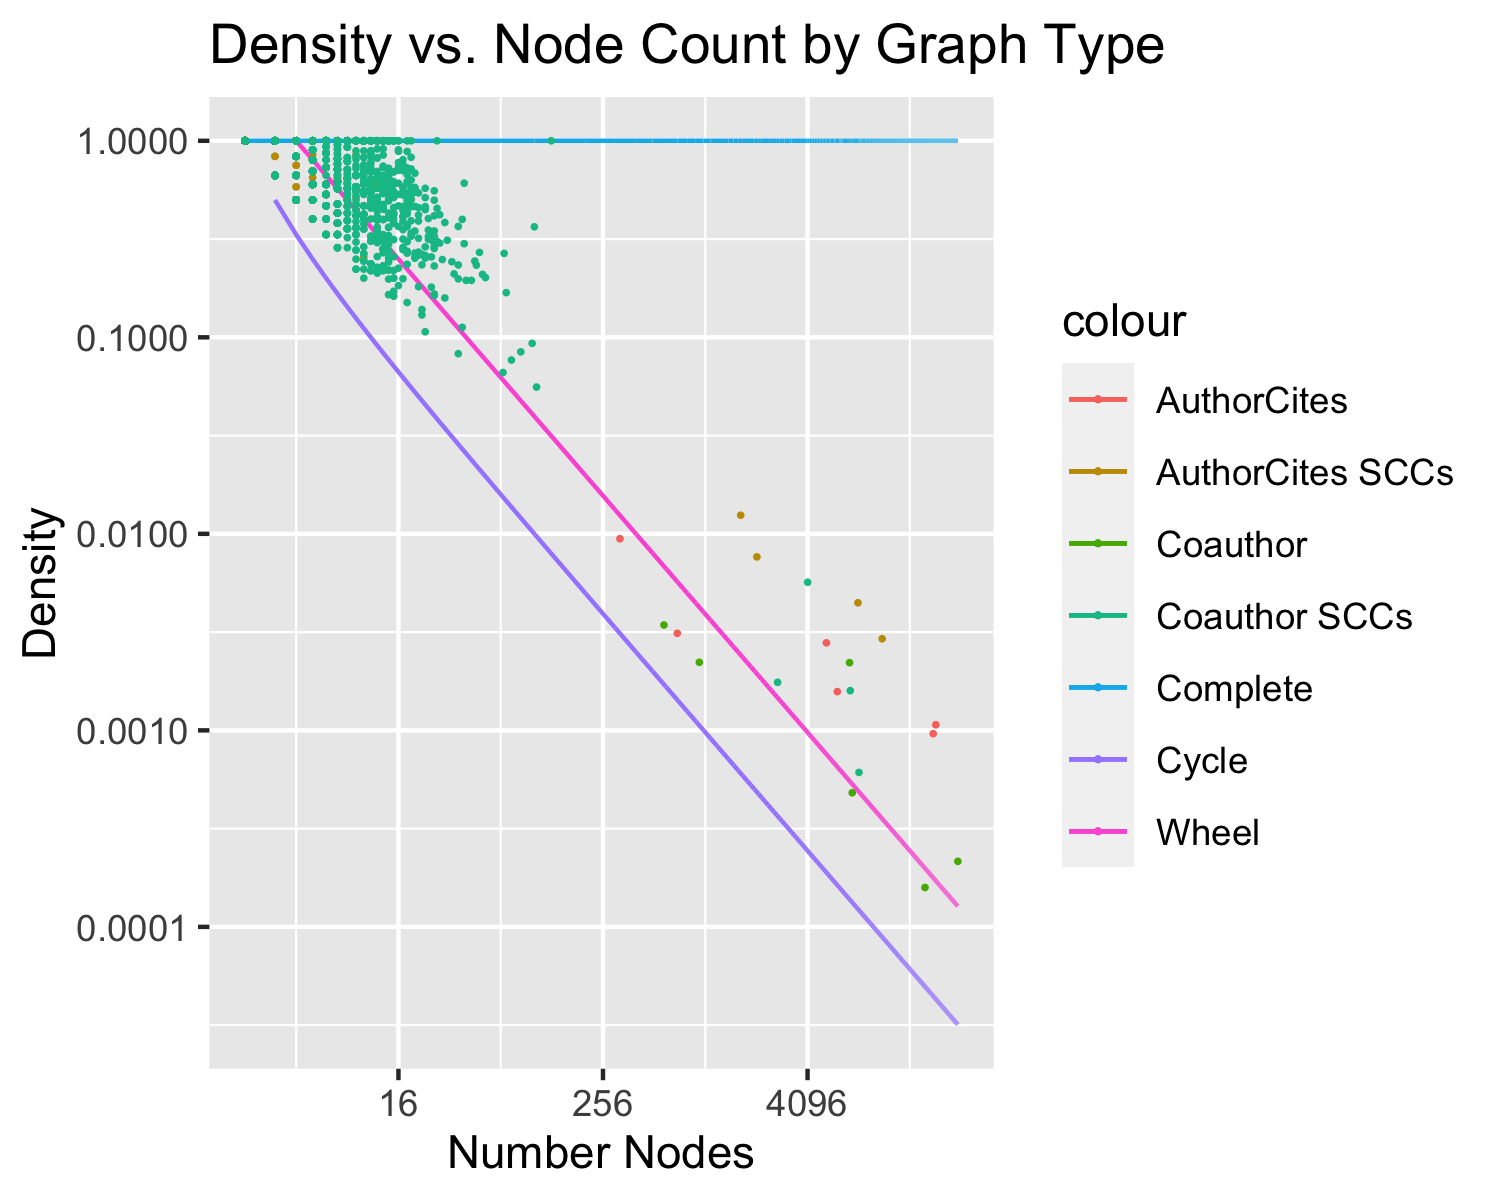
\includegraphics{figures/node_density_plot.png}
\caption{\(\log\) plot of graph density vs.~the number of nodes. Note
that the empirically constructed strongly-connected components decline
in density as they grow in size. This effect causes them to diverge from
the structure of complete graphs and begin to look much more like denser
versions of the cycle and wheel graphs.}\label{fig:nodesvdensity}
}
\end{figure}

Next, I decided to use a classic measure of graph structure, the degree
distribution, to show another critical way these . For the cycle and
complete graphs, every node either has two neighbors or \(n\) neighbors
for a graph of size \(n\). A wheel's edge nodes each have three
neighbors and the central node has \(n-1\) neighbors. This means the
degree of each node, the count of neighbors, doesn't vary from node to
node, which is a striking difference compared to real citations patterns
\ref{fig:degdist}.

\begin{figure}
\hypertarget{fig:degdist}{%
\centering
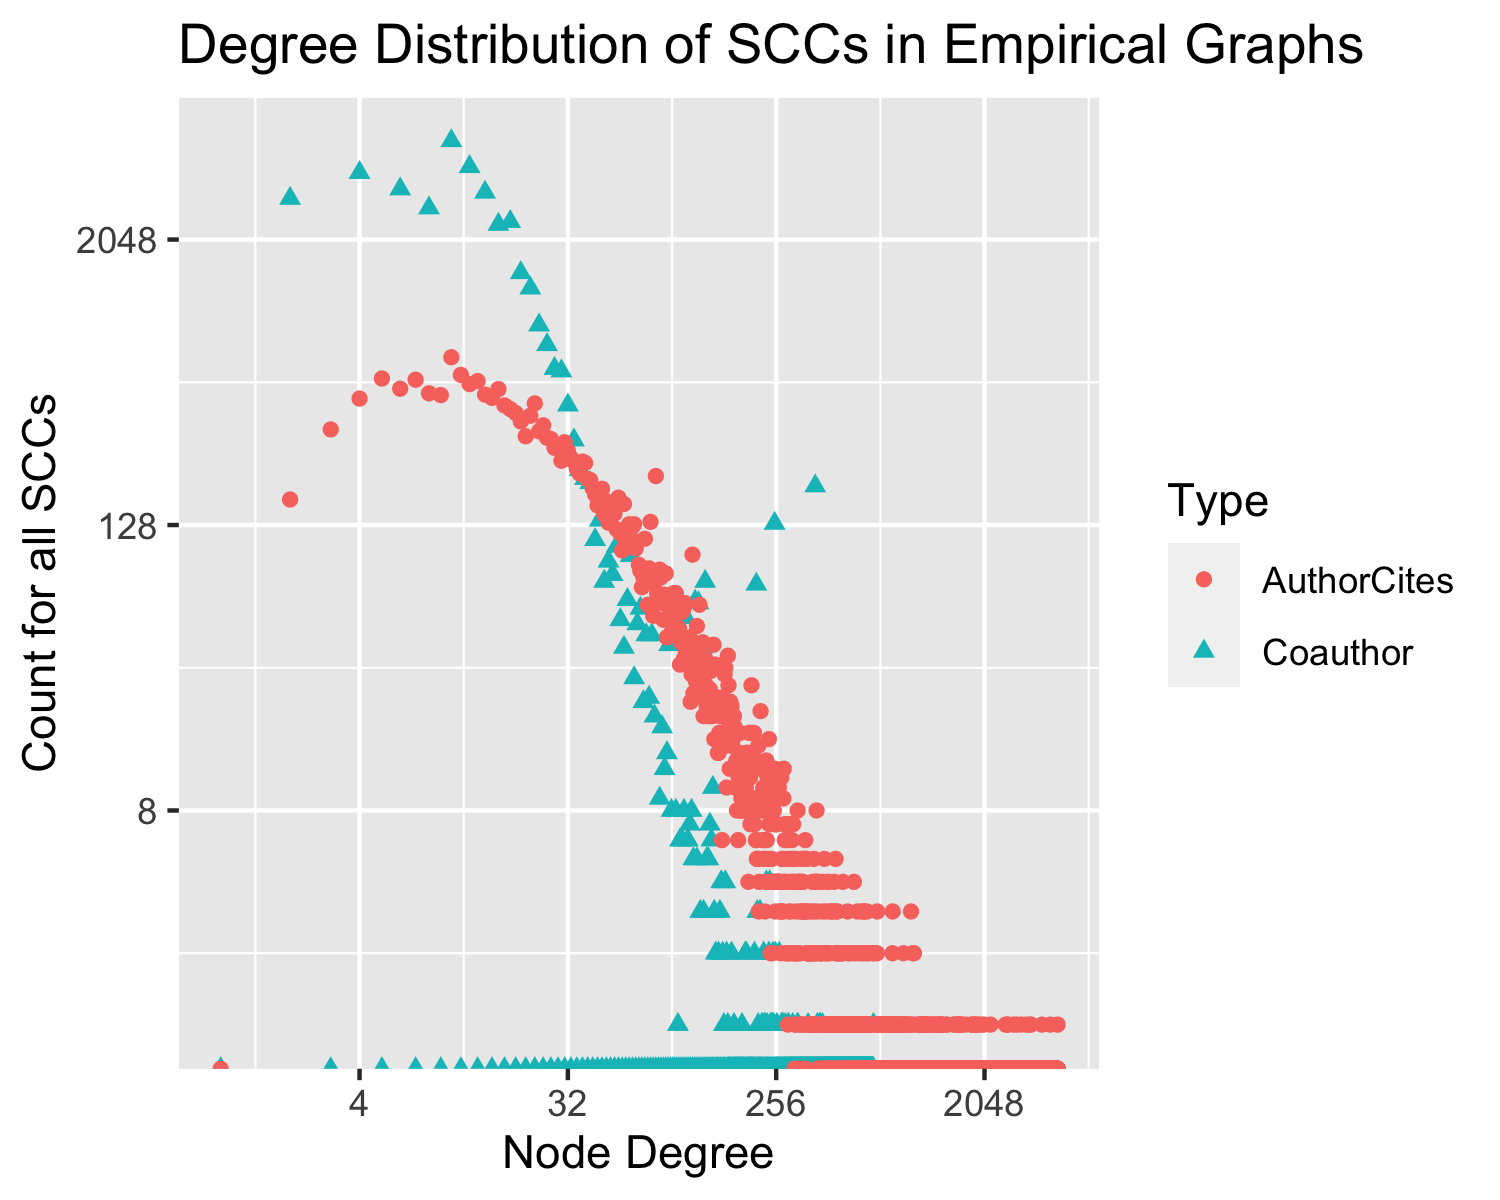
\includegraphics{figures/scc_degree_distribution.png}
\caption{\(\log\)-\(\log\) plot of degree distributions for empirical
SCC node degree counts that shows both AuthorCites and CoAuthor networks
roughly follow a power-law degree distribution. For context, cycle and
complete graphs are populated entirely with nodes with precisely the
same degree whereas, in the wheel graph, all but the central node has
the same degree. Thus, the citation graphs have distinctive diversity in
degree distribution compared with these synthetic
graphs.}\label{fig:degdist}
}
\end{figure}

Instead, this power-law distribution of real citation is what is often
called a ``small world'' distribution. These sorts of networks are
structure such that no two nodes are more than a few ``steps'' away from
each other, despite a lack of direct connections. The idea here is that
while you might have a small group of direct friends, the friends of
friends group and friends of friends of friends groups can be quite
large, encompassing many people thought to be complete strangers. The
conclusion to draw from this power-law effect is that this property is a
distinctive property of the graphs that is approximated, but not
replicated by any of the theoretical graphs.

\hypertarget{replicating-model-results}{%
\section{Replicating Model Results}\label{replicating-model-results}}

Now, given these graphs are notably different, how does Zollman's model
stack up on them? Do they behave like any of the synthetic graphs and,
if so, which ones? Furthermore, given that these graphs represent actual
communities, does the Zollman's noted effect where some denser
communities converge at a lower rate apply?

To begin to answer these questions, I ran Zollman's simulations on the
strongly-connected components from the AuthorCites graphs. I did not run
the simulations on the CoAuthor network because the co-authorship
relation does not map to communication in the sense that Zollman is
talking about. Collaboration is distinct from communication and Zollman
discusses the latter. Recall that in Zollman simulations, the model is
marked as ``converged'' successfully if and only if all agents chose the
action with a higher probability of success after the final model
iteration. Because this varies from run to run based on different random
seeds, Zollman often carries out repeated runs to approximate the
probability that the agents all converge.

To visualize the results of these simulations, I first plotted Zollman's
convergence metric relative to the density of the AuthorCites
strongly-connected components in figure \ref{fig:convergeprobdensity}.
This figure revealed that the same density-dependence relation Zollman
established still holds here. The least-dense real-world communities had
the highest probability of successful convergence on simulations.
However, the least-dense social network graphs are the largest ones. For
example, the field of peptic ulcer research contains a large strongly
connected component of low density that converged to the action with the
highest inherent probability of success on nearly every trial. Recall
that Zollman exhibited the field of peptic ulcer research as an example
of premature convergence leading to the wrong outcome. Thus, while
Zollman might have discovered a potential problem with a potential
solution in his models, the mechanisms in the model that led to that
problem seem notably different than those at play in these real-world
communities. For context, the large real-world communities converge
successfully with the same probability that Zollman observed in less
connected graphs.

On the other hand, there do exist many small groupings of 5-20 authors
that converge at lower rates due to high density. However, these
groupings don't have the influence that larger strongly-connected
components do because, by definition, they are not cited by anyone in
the primary connected component that makes up the bulk of the field in
most cases. This could be an interesting point for further structural
investigation of different fields as these smaller groupings have very
different structural properties than the larger graphs. Many of them are
nearly complete graphs. This could be due to a number of factors, such
as lab groupings which cause people to cite within a lab, lineages of
certain collaborations, etc. Determining why these are the case and
their prevalence in different fields of research would require more
careful empirical work by reading the papers involved and determining
what factors led to that structure. Deeper understanding here could help
shed light on how fragmented different fields are and what causes that
fragmentation.

\begin{figure}
\hypertarget{fig:convergeprobdensity}{%
\centering
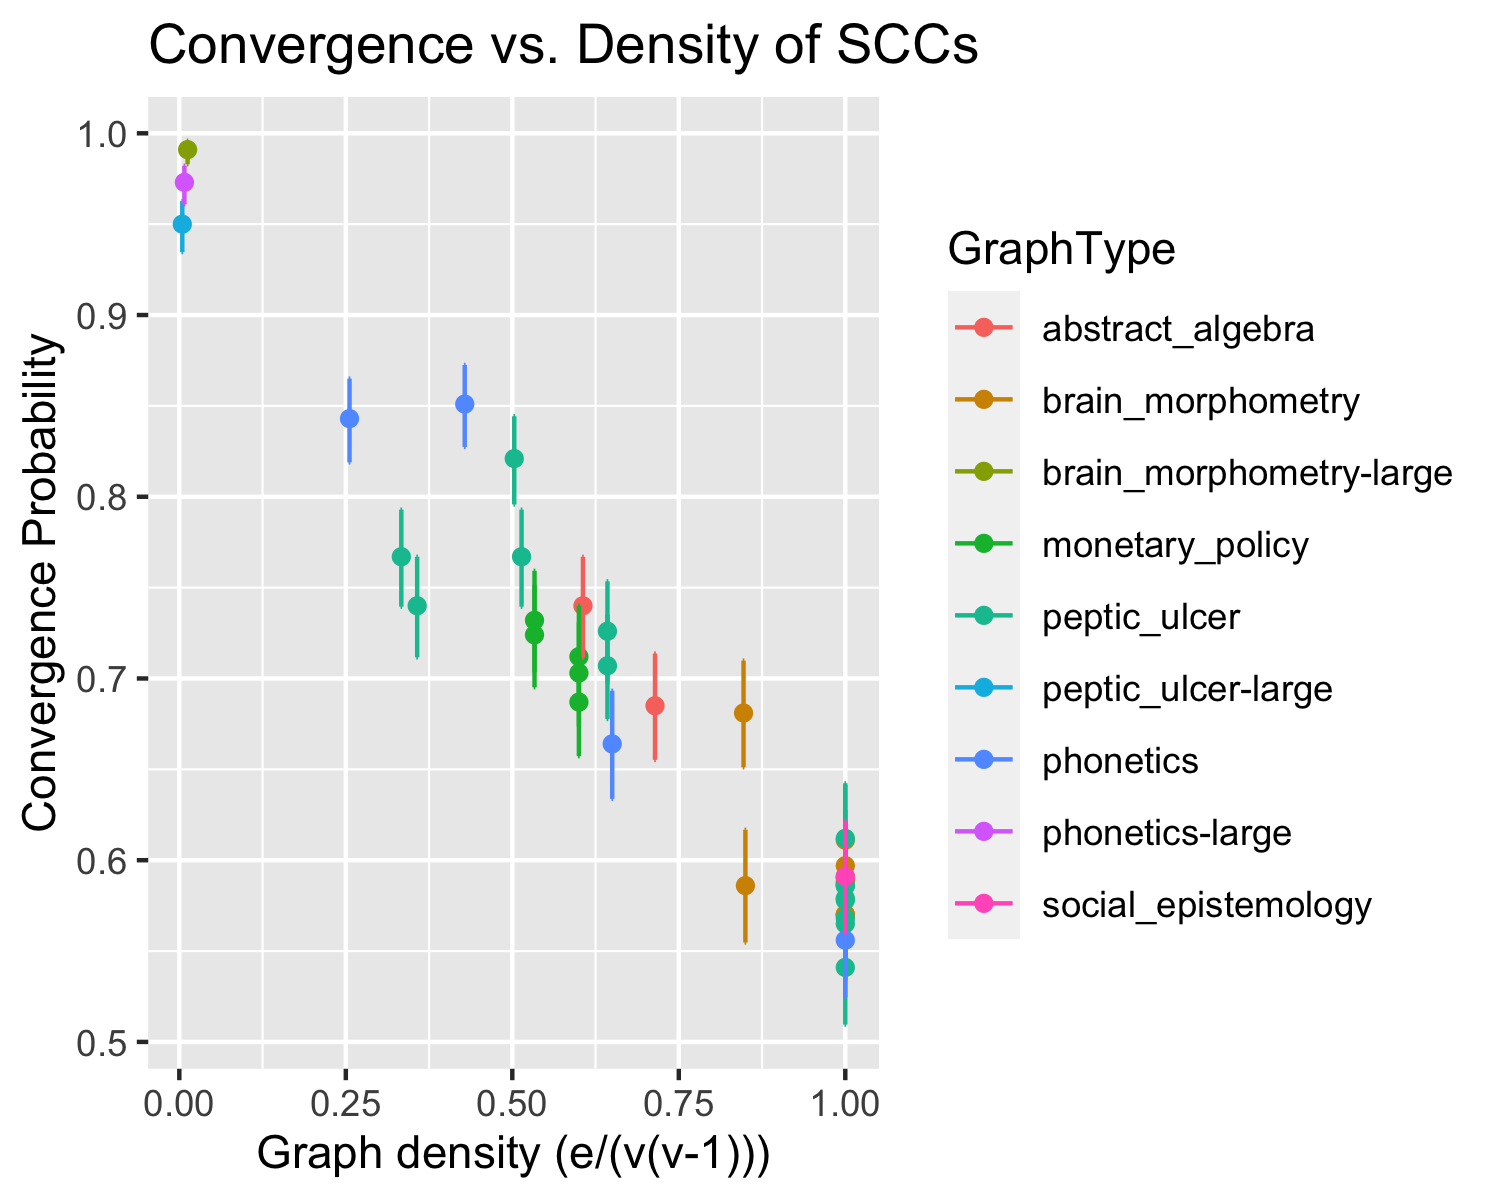
\includegraphics{figures/converge_prb_density.png}
\caption{Plot of successful convergence probability, as defined by
Zollman, against density for model runs on AuthorCites strongly
connected components. Graphs with more than 150 nodes are marked as
large. Note that all such large graphs are in the very top left corner
and have notably higher convergence probability. Each point has an
associated 95\% binomial confidence interval computed using the set of
trials.}\label{fig:convergeprobdensity}
}
\end{figure}

Next, I turned my attention to how fast the models converged on larger
graphs and what fraction of nodes end up selecting the right action at
each step. Do larger graphs converge more quickly? What fraction of
nodes get it right or wrong in the end? In figure
\ref{fig:convergespeed}, we see that large graphs converge very quickly
and completely, with very little variation in the fraction of nodes that
end up converged. Smaller graphs, on the other hand, have quite a bit
more variation partly because a single incorrect node has a bigger
impact on the overall network when that network is small. One node wrong
in four is a major schism whereas one node wrong in two-thousand is an
outlier.

\begin{figure}
\hypertarget{fig:convergespeed}{%
\centering
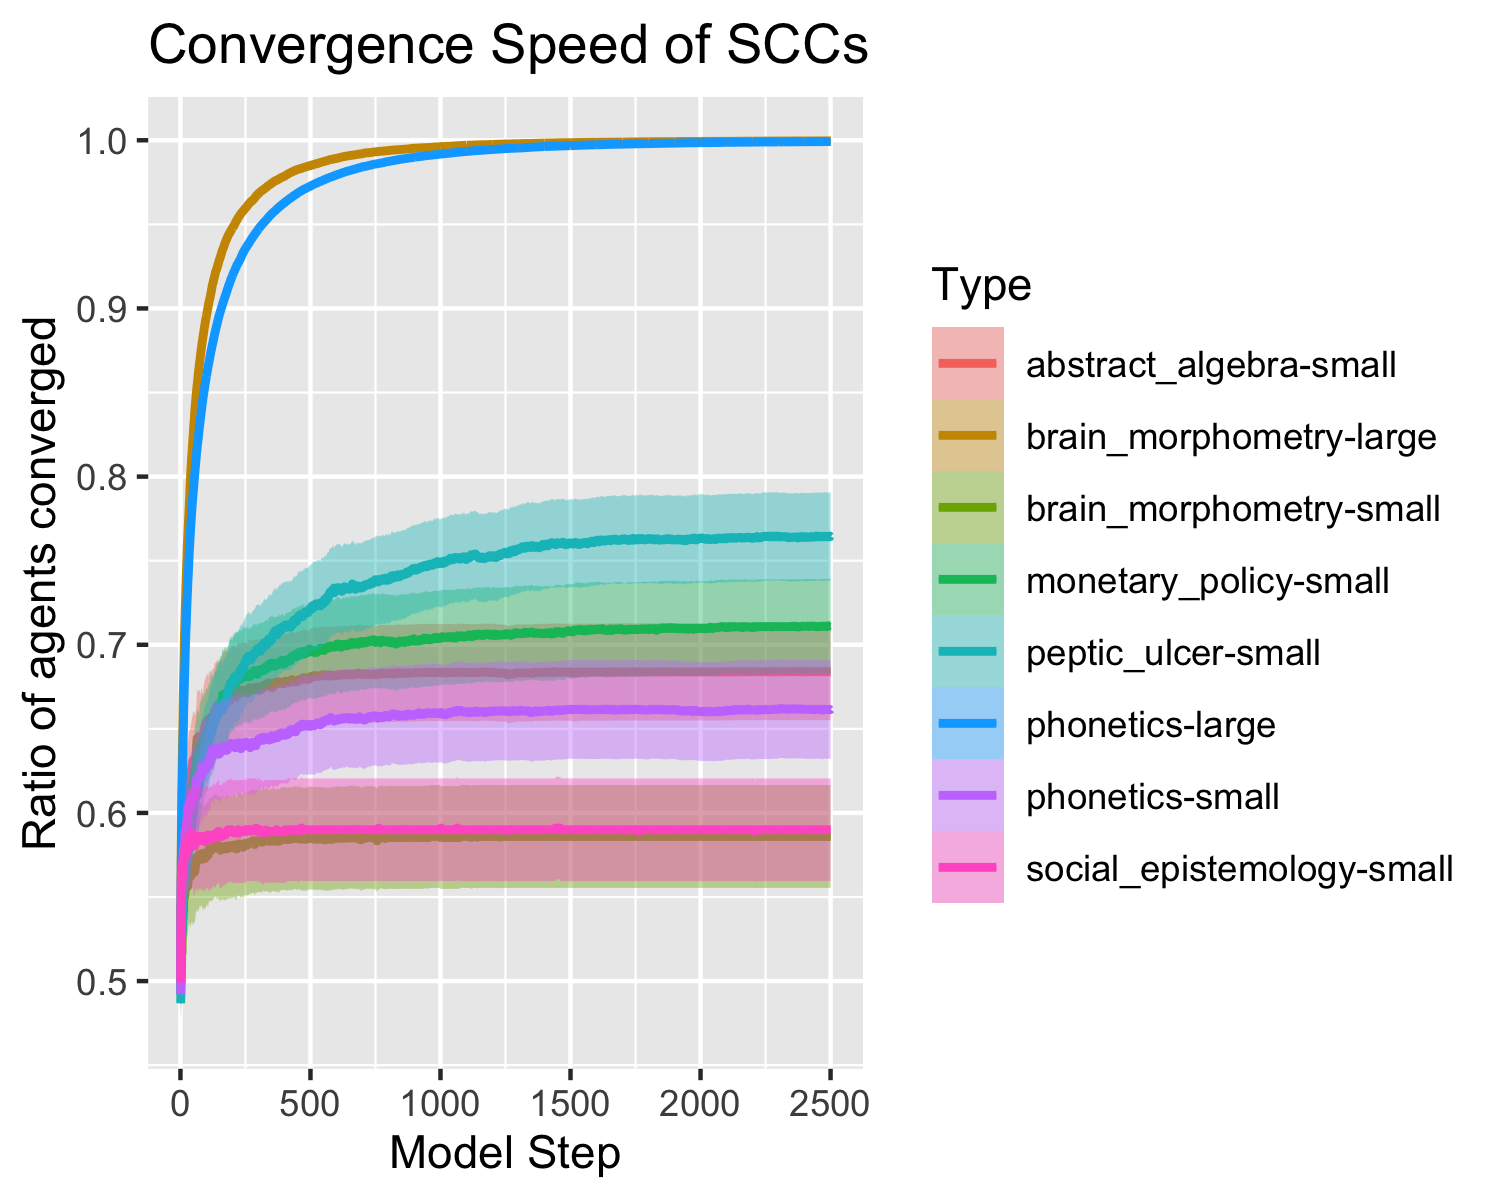
\includegraphics{figures/converge_speed.png}
\caption{Graph showing the convergence by step. The lines shown are the
mean ratio of agents converged at that given step with a 95\% confidence
interval shown as a band around each line. Very large, sparse graphs
quickly converge to complete agreement. Small dense graphs converge more
slowly to a plateau. The mean and confidence interval metric does not
capture that smaller graphs also jump out of that plateau and converge
rapidly when then do converge, though that happens at a much lower rate
that the large graphs.}\label{fig:convergespeed}
}
\end{figure}

\hypertarget{characterizing-model-behavior}{%
\section{Characterizing Model
Behavior}\label{characterizing-model-behavior}}

While the graphs of convergence probabilities and densities quantify the
behavior of the model and allow for rigorous conclusions, they don't
give a good intuitive idea of what a model \emph{looks} like. To rectify
this, figure \ref{fig:pepticprog} presents a pictorial view of a single
model run of the simulation on the peptic ulcer graph. To do this, I
used the standard ``spring'' layout algorithm to visualize the graph
structure and recolored each node according to its selected action at
each step. Nodes can be seen slowly flipping back and forth between the
two actions but the simulation eventually converges and all agents agree
on the right action. This happens rapidly because the peptic ulcer graph
is large and sparse. The spring layout shows that one part of peptic
ulcer work is denser than the other and thus that dense core converges
slightly faster than the rest of the graph before propagating out to all
nodes at the peripheries. Nodes in the middle generally have a higher
degree while nodes at the edges have a lower degree, so this is
consistent with the most well-connected authors converging first to a
new trend with less connected authors adopting that theory much later.

\begin{figure}
\hypertarget{fig:pepticprog}{%
\centering
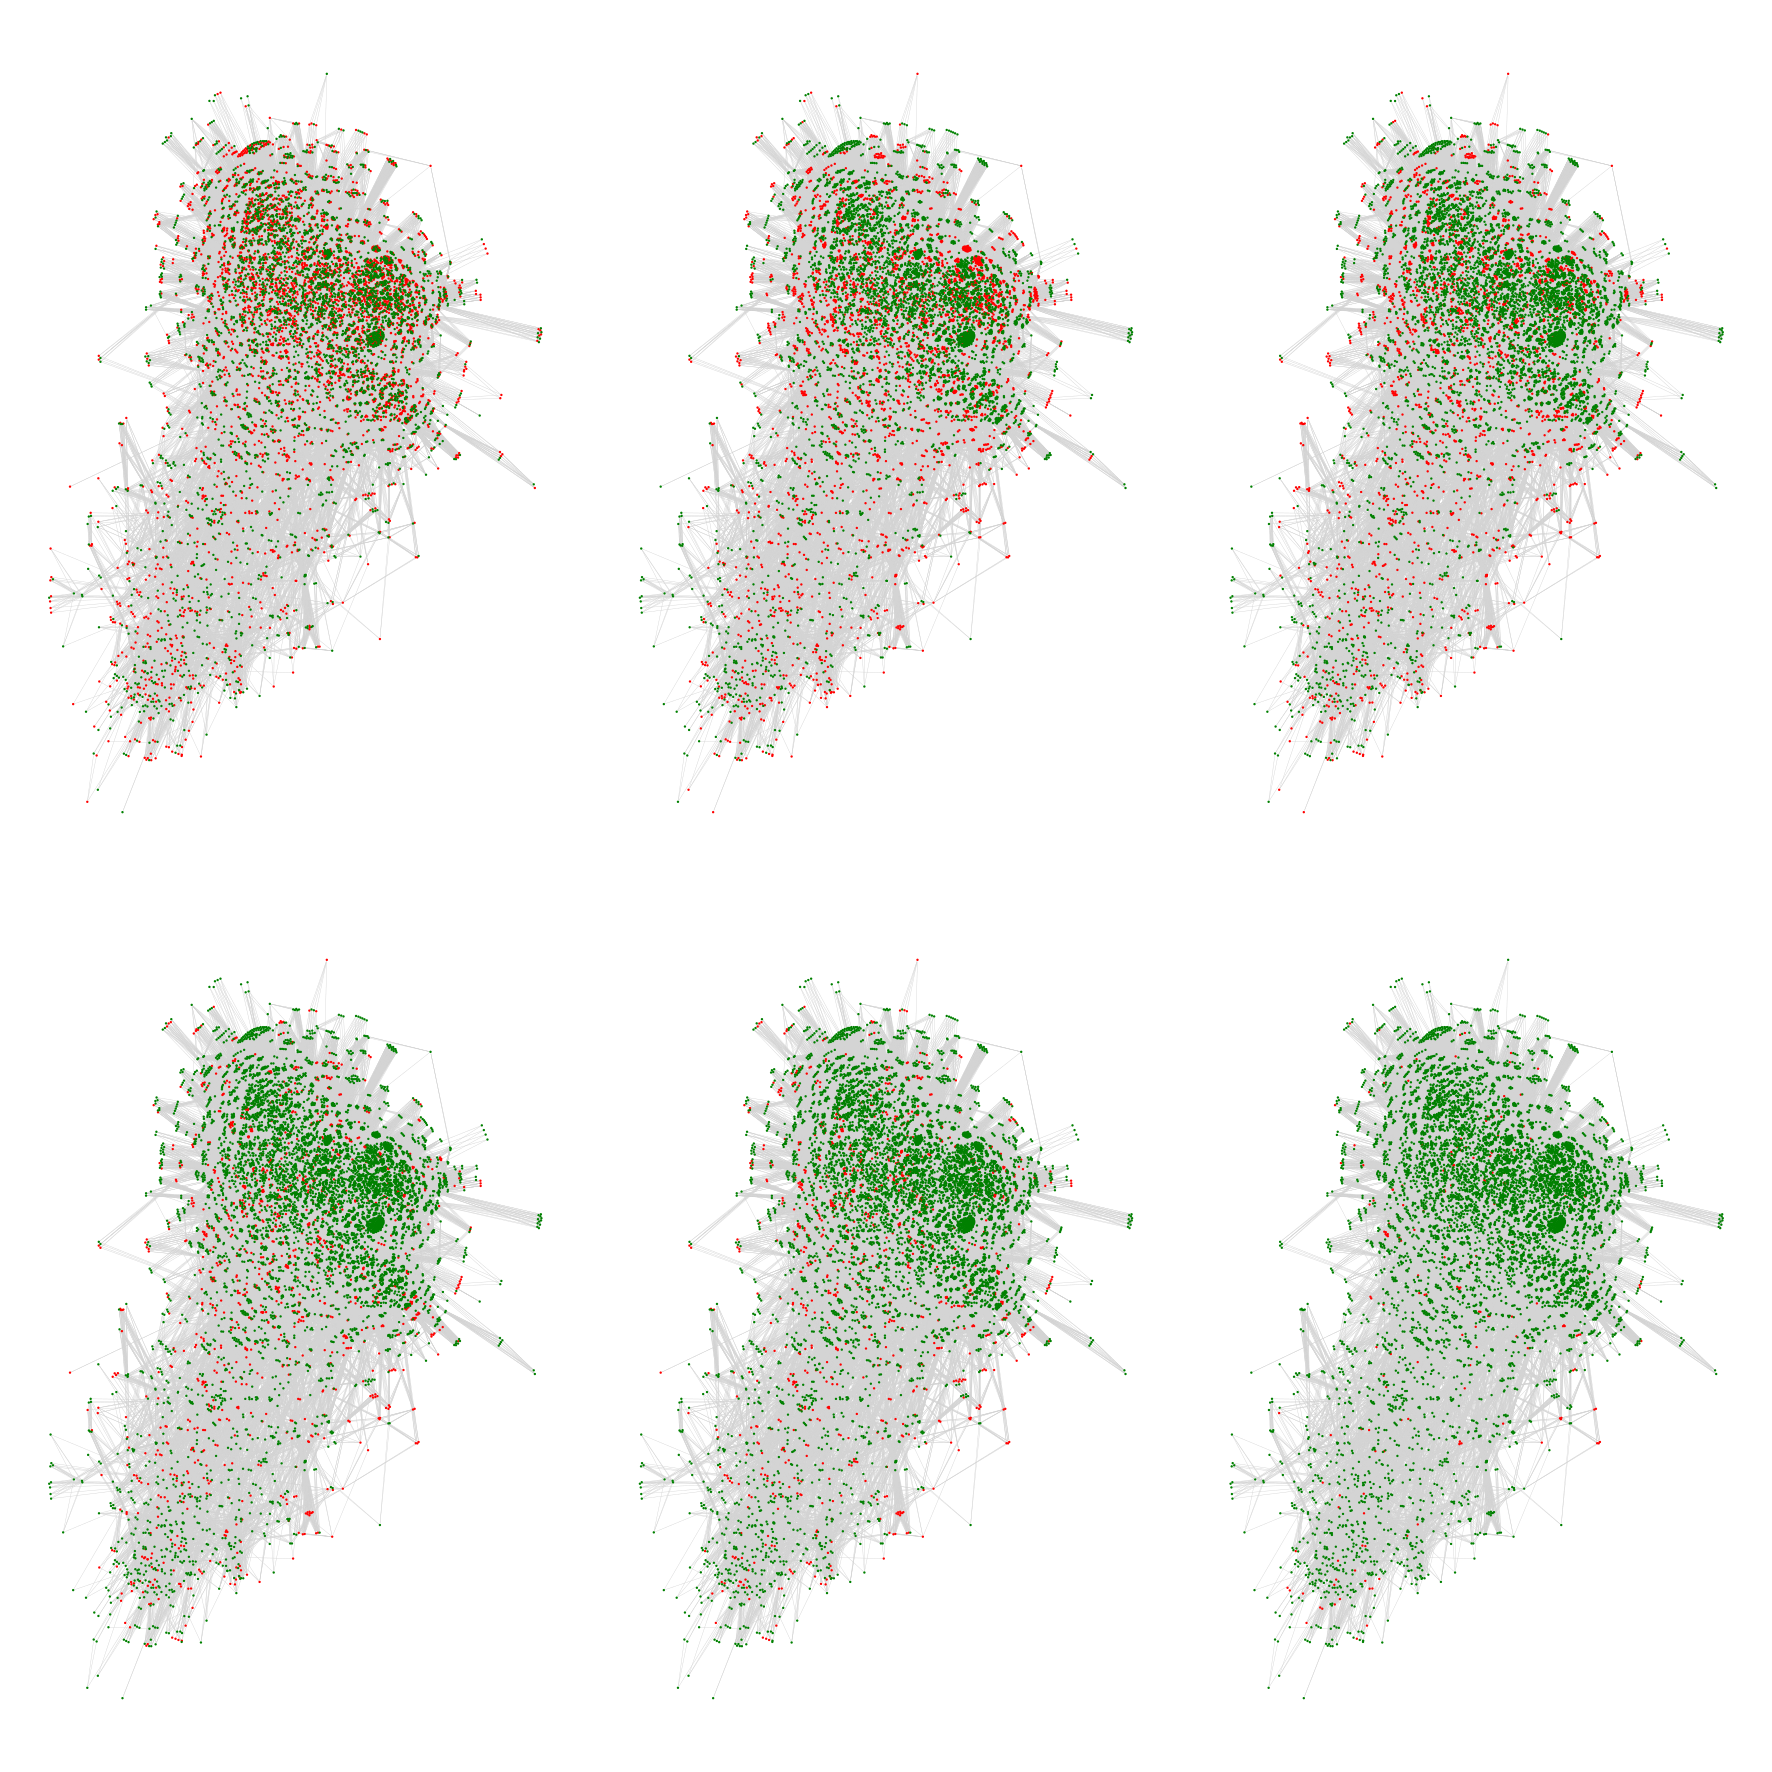
\includegraphics{figures/peptic_ulcer_1-5-10-50-100-500.png}
\caption{Frames from a model run on the large peptic ulcer strongly
connected component. Each plot shows that state of the model at a given
step where red nodes have chosen the suboptimal theory and green nodes
the optimal one. The first row contains the initial state, the state
after the 5th step and the one after the 10th. The second has the 50th,
the 100th, and the 500th. The simulation continues on to 10,000 steps
where all nodes are green, but nearly all nodes have chosen correctly by
step 500 on the peptic ulcer graph because it is large and
sparse.}\label{fig:pepticprog}
}
\end{figure}

\hypertarget{experimental-conclusions-and-takeaways}{%
\section{Experimental Conclusions and
Takeaways}\label{experimental-conclusions-and-takeaways}}

Overall, the empirically-simulated models largely converged at rates
that Zollman's findings would have predicted based on the
graph-theoretic properties of the AuthorCites graphs. Lower density
graphs converged more completely than higher density ones, which is
consistent with Zollman's findings. However, the large, less-dense
graphs also converged faster than their denser counterparts, which calls
into question one of Zollman's worries: that less density and less
communication can lead to slower convergence which delays science.

In reality, these less dense graphs are substantially less dense than
any complete graph, but are much denser than the cycle and wheel graphs
that Zollman tests against. The ``small world'' effect also means that
pair-wise distances between nodes are short and thus information never
has that far to travel between nodes. This effect differs quite a bit
from the cycle graph which forces agents to play telephone with their
results, slowing convergence substantially.

Most importantly, these results call into question Zollman's
recommendation for less communication to avoid premature convergence.
The answer must be much more nuanced than this given these results.
First of all, the scholarly graphs are for the most part not that dense
already and they converge at high rates as Zollman predicts. Secondly,
they also happen to converge faster than small dense graphs, indicating
that there is no price paid for that high rate of successful
convergence. In short, real-world ``small world'' graphs get the best of
both worlds under Zollman's metrics.

However, this means that these effects cannot explain why the peptic
ulcer field converged prematurely because that field is fairly well
structured for Zollman's model. Zollman's model would predict that
problematic fields like peptic ulcer research would be too dense and
converge to the wrong answer too quickly. However, because the peptic
ulcer graph turned out to not be very dense, it converged quickly to the
right answer, meaning the Zollman's model doesn't explain why peptic
ulcer research in the real world converged on the wrong answer. Thus,
some other mechanism than the one modeled must be at play.

Furthermore, there is a sense in which the problem here is not enough
communication. For example, the strongly connected components that were
small and very dense can counterintuitively lower the overall density of
the large graph by joining it. This means that had some of those dense
components joined the larger, primary component of the field, the field
likely would maintain the same fast and accurate convergence that the
larger component had from the start. Thus, the answer cannot be as
simple as a blanket recommendation of less or more density, rather, some
groups who are separated from the overall community might benefit from
being looped in with the mainstream. Furthermore, those in the
mainstream would do better by reaching out and forming new connections
with these disconnected groups than by densifying the large central
component further.

So, this empirical work suggests the while Zollman's theoretical results
hold, their application to real data changes our understanding of what
those results mean for the actual world. Because I wanted the comparison
with Zollman's work to be direct, I mirrored his model structure exactly
but for the empirical graphs. This highlights how empirical grounding
changes conclusions, however, it also means my work likely suffers from
all the same mathematical stability problems identified by Rosenstock,
Bruner, and O'Connor \autocite{rosenstockEpistemicNetworksLess2017a}.
Essentially, the model is not robust to changes in non-graph parameters,
like the underlying binomial probabilities of the actions and the
initial priors for each individual. An interesting follow-up project
might be to determine if this sensitivity is reduced to some extent on
the more robust ``small world'' graphs.


\hypertarget{conclusion}{%
\chapter{Conclusion}\label{conclusion}}

To conclude this thesis, I'll spend a bit of time ruminating on how
these empirical methods were useful and how they could be applied
elsewhere. To do this, I'll talk a bit about how they differ from the
robustness analysis that already done in computational modeling. To do
this, I'll paint a picture that explains when each of these tools should
be used and why. Both of these tools are designed to show that a
simulation result is robust and applies to the real world, though they
do it in very different ways.

First, I'll introduce the strategy employed by Rosenstock, Bruner, and
O'Connor \autocite{rosenstockEpistemicNetworksLess2017a}. They performed
a robustness analysis over many of the non-graph parts of the model and
found that for many choices, Zollman's results don't hold up. They
conclude that because the parameter space is large and only a very small
part of it results in Zollman's observed effect that the effect is
unlikely to occur in the real world. Overall, robustness analysis is a
very useful strategy to understand the limitations of a given model
because it helps to show in much more detail what interplay there is
between parameters. It also has the potential to identify very robust
effects that would be much more likely to apply in the real world. If
the effect holds for all parameter values, then it seems fairly likely
that the real world parameter values fall into that range! On the other
hand, as in the Zollman case, if the parameters need to be fine-tunned
to observe the effect, we'd need the parameters for the world to also be
fine-tunned in the same way for the model to apply to the real world.
Concretely, the O'Connor work most usefully identifies that the
probabilities of each action must be \emph{very} close together to get
any sort of trade-off at all. If they are even slightly further apart,
the model converges at a high rate no matter the priors or the
structure. Thus, if all the choices of action have very similar chances
of success, then the effects observed in this thesis likely still hold.
If they are further apart, more work would need to be done to see if
this sensitivity persists on the large social graphs.

Empirically-backed models try to show that a model generalizes in a very
different way. Where robustness analysis asks does this hold for all
parameters, empirical work asks does this hold for a few very
representative parameter values. The reality is that the world often
isn't robust to parameter changes so robustness analysis alone cannot
account for all phenomena in the world. For example, there are many
physical constants in the universe that, if perturbed slightly, would
make life as we know it unimaginable. There has been much debate over
what this means and the implications of it, recently over things like
the Anthropic principle or intelligent design in cosmology. However,
that doesn't change the fact that lack of robustness is a striking
feature of the world we live in.

Thus, empirical methods allow us to learn how well a model applies to
the real world by simply using real-world parameter values. This
requires data collection work analysis and understanding that isn't
present for all aspects of the world, however, for many we do know the
parameters pretty well. For example, an engineering simulation of a
bridge on earth need not be robust to changes in the Earth's gravity
because we know that parameter to be fixed to a certain value
(\(10 m/s^2\)).

My work here does a similar thing for social networks. Because of the
extensive empirical work cataloging citations, we now have a very
comprehensive proxy which captures one important dimension of scientific
community structure. This citation structure is fairly fixed and stable
in the sense that people can only keep up with and cite the work of a
certain number of others and some people will always turn out to be more
influential than others due to media coverage, social media, etc. Thus,
models which deal with this structure only need to be robust to
variations that could feasibly occur. So a robustness analysis that
shows the model doesn't hold for cycles doesn't tell us much because
people never organize themselves in cycles except to play the game
``telephone''.

The Rosenstock, Bruner, O'Connor piece, however, does focus on
parameters that are unique to the model and not present in the real
world. This means we necessarily don't have good priors on them in the
same way we do for social network structure. Thus, a robustness analysis
is all that is possible. We don't know at all how far apart action
probabilities are in the real world because it is unclear what those
action probabilities map to in the first place. We don't know what a
reasonable initial beta distribution for belief about those actions is
either because we don't know exactly how people form prior beliefs about
the lines of work they go into. Thus, in these cases, robustness
analysis has to fill the gaps. However, ideally, we would like to
understand and observe the mechanisms at play in the real world so we
can better calibrate our models.

At the end of the day, the parameter space that matters is the one for
the real world in which we live, which is much smaller than the set of
mathematically possible parameters in many cases. Pushing for narrowing
the parameter space to what exists in the real world often elucidates
interesting results because that smaller parameter spaces can be more
thoroughly explored. My work here showed that the real world parameter
space had quite different properties than the more generalized and
idealized parameter space which Zollman tried to use in exploring the
parameter space of graph structure.

Thus, in addition to my results extending Zollman's model, this work
shows that empirical analysis within computational philosophy can be a
critical tool in addition to robustness analysis. While not possible for
every aspect modeled, finding empirical priors contextualized the model
results to a parameter space that, by definition, reflects some part of
reality. Sometimes, and as was the case with Zollman, this smaller
parameter space can shine some light on the peculiarities of our world.
For example, the fact that more communication can lead to less overall
density when an isolated community engages with the mainstream.
Philosophers would be privy to define their theories in terms of good
empirical priors wherever possible to sharpen their arguments and to
ensure that those arguments actually go through for the complicated and
rich world in which we live in.


\appendix

\hypertarget{code-and-data}{%
\chapter*{Code and Data}\label{code-and-data}}
\addcontentsline{toc}{chapter}{Code and Data}

The Julia code for my core simulation can be found at:

\url{https://github.com/jackbeasley/NetworkEpistemology.jl}.

\noindent The datasets, figures, and experimental code can be found at:

\url{https://github.com/jackbeasley/NetworkEpistemology-Thesis-Experiments}

\noindent The fast Microsoft Academic Graph to neo4j CSV converter can
be found at:

\url{https://github.com/jackbeasley/mag-csv}


\printbibliography

\end{document}